\documentclass{beamer}\usepackage[]{graphicx}\usepackage[]{color}
%% maxwidth is the original width if it is less than linewidth
%% otherwise use linewidth (to make sure the graphics do not exceed the margin)
\makeatletter
\def\maxwidth{ %
  \ifdim\Gin@nat@width>\linewidth
    \linewidth
  \else
    \Gin@nat@width
  \fi
}
\makeatother

\definecolor{fgcolor}{rgb}{0.345, 0.345, 0.345}
\newcommand{\hlnum}[1]{\textcolor[rgb]{0.686,0.059,0.569}{#1}}%
\newcommand{\hlstr}[1]{\textcolor[rgb]{0.192,0.494,0.8}{#1}}%
\newcommand{\hlcom}[1]{\textcolor[rgb]{0.678,0.584,0.686}{\textit{#1}}}%
\newcommand{\hlopt}[1]{\textcolor[rgb]{0,0,0}{#1}}%
\newcommand{\hlstd}[1]{\textcolor[rgb]{0.345,0.345,0.345}{#1}}%
\newcommand{\hlkwa}[1]{\textcolor[rgb]{0.161,0.373,0.58}{\textbf{#1}}}%
\newcommand{\hlkwb}[1]{\textcolor[rgb]{0.69,0.353,0.396}{#1}}%
\newcommand{\hlkwc}[1]{\textcolor[rgb]{0.333,0.667,0.333}{#1}}%
\newcommand{\hlkwd}[1]{\textcolor[rgb]{0.737,0.353,0.396}{\textbf{#1}}}%
\let\hlipl\hlkwb

\usepackage{framed}
\makeatletter
\newenvironment{kframe}{%
 \def\at@end@of@kframe{}%
 \ifinner\ifhmode%
  \def\at@end@of@kframe{\end{minipage}}%
  \begin{minipage}{\columnwidth}%
 \fi\fi%
 \def\FrameCommand##1{\hskip\@totalleftmargin \hskip-\fboxsep
 \colorbox{shadecolor}{##1}\hskip-\fboxsep
     % There is no \\@totalrightmargin, so:
     \hskip-\linewidth \hskip-\@totalleftmargin \hskip\columnwidth}%
 \MakeFramed {\advance\hsize-\width
   \@totalleftmargin\z@ \linewidth\hsize
   \@setminipage}}%
 {\par\unskip\endMakeFramed%
 \at@end@of@kframe}
\makeatother

\definecolor{shadecolor}{rgb}{.97, .97, .97}
\definecolor{messagecolor}{rgb}{0, 0, 0}
\definecolor{warningcolor}{rgb}{1, 0, 1}
\definecolor{errorcolor}{rgb}{1, 0, 0}
\newenvironment{knitrout}{}{} % an empty environment to be redefined in TeX

\usepackage{alltt}
\usetheme{default}
%\usetheme{Malmoe}

\title[EC999: Quantitative Text Analysis]{EC999: Text Normalization} \def\newblock{\hskip .11em plus .33em minus .07em}


\def\Tiny{\fontsize{10pt}{10pt}\selectfont}
\def\smaller{\fontsize{8pt}{8pt}\selectfont}

\institute[Warwick]{University of Chicago \& University of Warwick}
\author[Thiemo Fetzer]{Thiemo Fetzer}

 \date{\today}

\usepackage{natbib}
\usepackage{amsmath}
\usepackage{hyperref}
\usepackage{graphicx}
\usepackage{graphics}

\usepackage{amsfonts}
\usepackage{amssymb}
\usepackage{pdfpages}
\usepackage{natbib}
\usepackage{hyperref}
%\usepackage{enumitem}
 \usepackage{pgffor}
\usepackage{booktabs,caption,fixltx2e}
\usepackage[flushleft]{threeparttable}
\usepackage{verbatim} 
\usepackage{cancel}
\newcommand\xxcancel[1]{\xcancel{#1}\vphantom{#1}}

\usepackage{mathtools,xparse}

\newenvironment{Description}
               {\list{}{\labelwidth=0pt \itemindent-\leftmargin
                        \let\makelabel\Descriptionlabel
                        % or whatever
               }}
               {\endlist}
\newcommand*\Descriptionlabel[1]{%
  \hspace\labelsep
  \normalfont%  reset current font setting
  \color{blue}\bfseries\sffamily% or whatever 
  #1}


\setbeamersize{text margin left = 16pt, text margin right = 16pt}
\newcommand{\code}[1]{\texttt{#1}}

\newenvironment<>{algorithm}[1][\undefined]{%
\begin{actionenv}#2%
\ifx#1\undefined%
   \def\insertblocktitle{Algorithm}%
\else%
   \def\insertblocktitle{Algorithm ({\em#1})}%
\fi%
\par%
\mode<presentation>{%
  \setbeamercolor{block title}{fg=white,bg=yellow!50!black}
  \setbeamercolor{block body}{fg=black,bg=yellow!20}
}%
\usebeamertemplate{block begin}\em}
{\par\usebeamertemplate{block end}\end{actionenv}}


\newenvironment<>{assumption}[1][\undefined]{%
\begin{actionenv}#2%
\ifx#1\undefined%
   \def\insertblocktitle{Assumption}%
\else%
   \def\insertblocktitle{Assumption ({\em#1})}%
\fi%
\par%
\mode<presentation>{%
  \setbeamercolor{block title}{fg=white,bg=blue!50!black}
  \setbeamercolor{block body}{fg=black,bg=blue!20}
}%
\usebeamertemplate{block begin}\em}
{\par\usebeamertemplate{block end}\end{actionenv}}

%changing spacing between knitr code and output
\usepackage{etoolbox} 
\makeatletter 
\preto{\@verbatim}{\topsep=0pt \partopsep=0pt } 
\makeatother
\renewenvironment{knitrout}{\setlength{\topsep}{0mm}}{}
\IfFileExists{upquote.sty}{\usepackage{upquote}}{}
\begin{document}



\AtBeginSection[]
{
 \begin{frame}<beamer>
 \frametitle{Plan}
 \tableofcontents[currentsection]
 \end{frame}
}
\maketitle
 

%%%%%%%%%%%%%%%%%%%%%%%%%%%%


%%%%%%%%%%%%%%%%%%%%%%%%%%%%%%%%%%%%%%%%%%%%%%%%%%%%%%%%%%
\begin{frame}[fragile]{Quantitative Text Analysis as process}
Above all, there needs to be a formulatedresearch question or \textbf{goal} to be achieved.
\begin{figure}[h]
\begin{center}
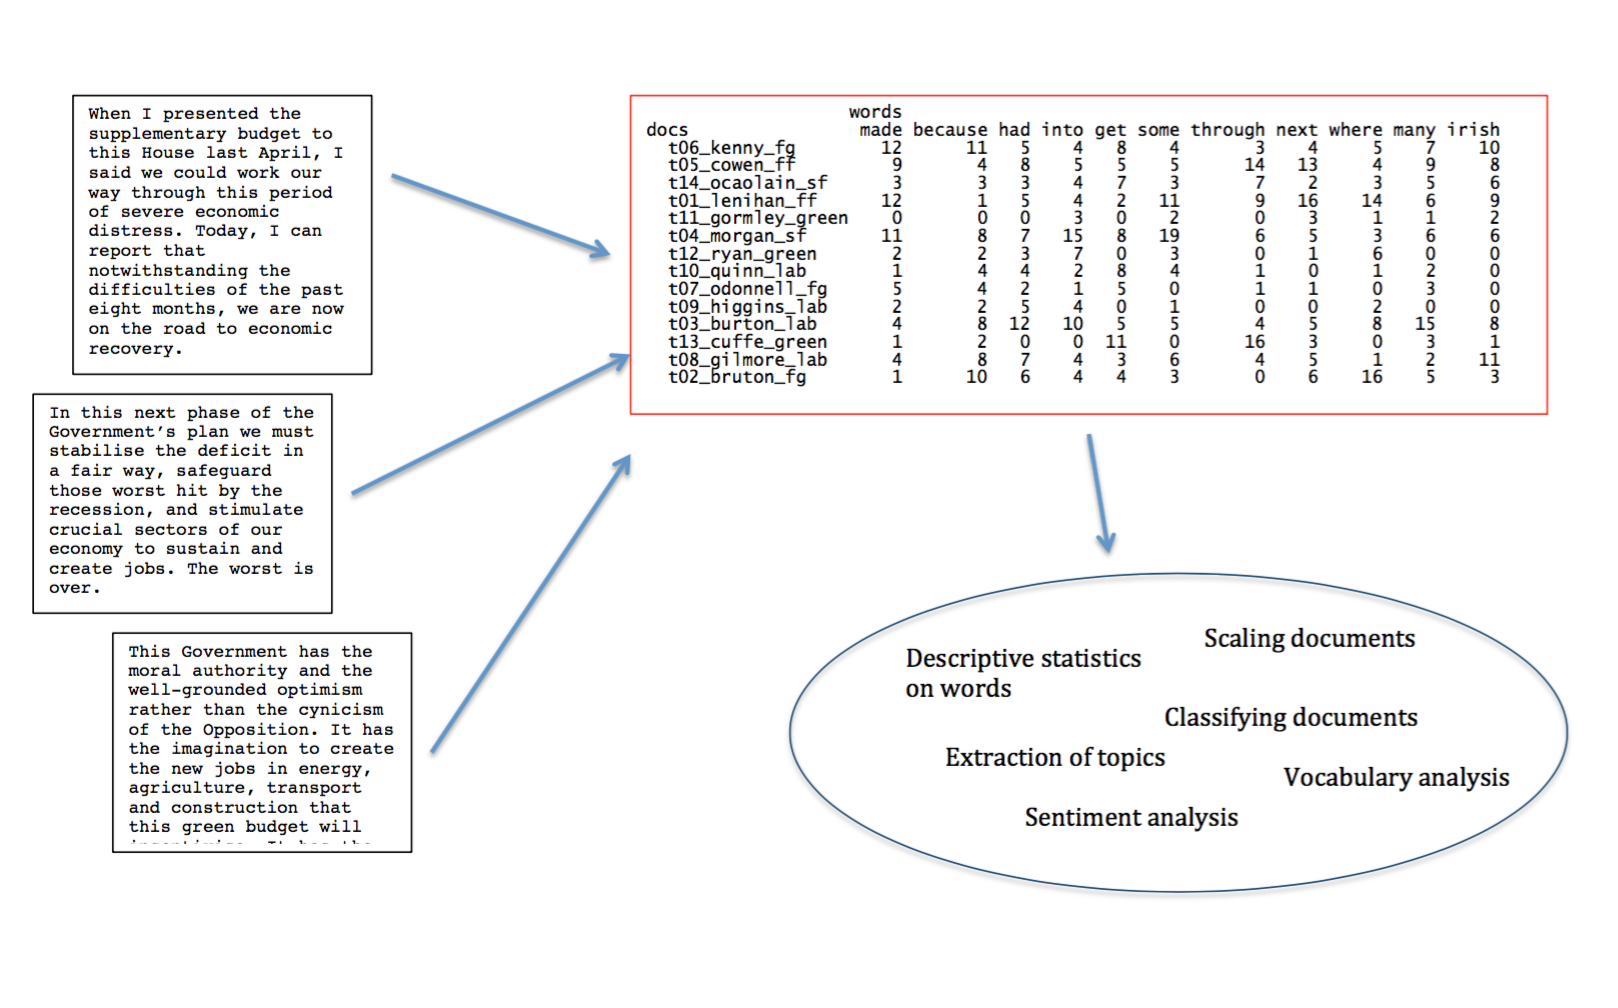
\includegraphics[scale=.4]{figures/qta-steps}
\end{center}
\end{figure}

\end{frame}
%%%%%%%%%%%%%%%%%%%%%%%%%%%%%%%%%%%%%%%%%%%%%%%%%%%%%%%%%%%%%%%%%%%%%%%%%

%%%%%%%%%%%%%%%%%%%%%%%%%%%%%%%%%%%%%%%%%%%%%%%%%%%%%%%%%%
\begin{frame}[fragile]{Building A Corpus}

\begin{itemize}

\item Textual data can be stored in multiple different formats

\begin{itemize}
\item JSON (JavaScript Object Notation) is a lightweight data-interchange format for structured data.
\item XML 
\item Flat text files
\item (machine readable?) PDFs
\end{itemize}

\item Parsing or reading text data into R can be achieved by a range of functions.
\end{itemize}

\begin{knitrout}\tiny
\definecolor{shadecolor}{rgb}{0.969, 0.969, 0.969}\color{fgcolor}\begin{kframe}
\begin{alltt}
\hlcom{#con can be any connection, could be a URL or a path to a file}
\hlstd{TEXT}\hlkwb{<-}\hlkwd{readLines}\hlstd{(}\hlkwc{con}\hlstd{=}\hlstr{"https://www.dropbox.com/s/eynnvac4kurnjon/speaches-2016-election.json?dl=1"}\hlstd{,} \hlkwc{encoding} \hlstd{=} \hlstr{"UTF-8"}\hlstd{)}
\hlcom{#commonly used for tabular data formats}
\hlstd{TEXT}\hlkwb{<-}\hlkwd{read.table}\hlstd{(}\hlkwc{file}\hlstd{=}\hlstr{"file.txt"}\hlstd{)}
\hlcom{#may need to iterate over a whole folder of documents}
\hlstd{TEST}\hlkwb{<-}\hlkwd{lapply}\hlstd{(}\hlkwd{list.files}\hlstd{(}\hlstr{"Path"}\hlstd{),} \hlkwa{function}\hlstd{(}\hlkwc{x}\hlstd{)} \hlkwd{readLines}\hlstd{(}\hlkwc{con}\hlstd{=x))}
\end{alltt}
\end{kframe}
\end{knitrout}

\end{frame}
%%%%%%%%%%%%%%%%%%%%%%%%%%%%%%%%%%%%%%%%%%%%%%%%%%%%%%%%%%%%%%%%%%%%%%%%%


%%%%%%%%%%%%%%%%%%%%%%%%%%%%%%%%%%%%%%%%%%%%%%%%%%%%%%%%%%
\begin{frame}[fragile]{An Example: Congressional speeches}

\begin{itemize}

\item Loading Congressional speaches by important figures important to the 2016 presidential election.
\item Data is JSON format
\item Each line is a speach given by a member of congress.
\item JSON data provides string excerpt as well as meta-information: date, party, speaker, chamber,...
\end{itemize}
\begin{figure}[h]
\begin{center}
\includegraphics[scale=.33]<1>{figures/json-speaches}
\end{center}
%\caption{\small{EU Enlargement in 2004}}
\end{figure}

\end{frame}
%%%%%%%%%%%%%%%%%%%%%%%%%%%%%%%%%%%%%%%%%%%%%%%%%%%%%%%%%%%%%%%%%%%%%%%%%



%%%%%%%%%%%%%%%%%%%%%%%%%%%%%%%%%%%%%%%%%%%%%%%%%%%%%%%%%%
\begin{frame}[fragile]{An Example: Congressional speaches}
\begin{knitrout}\tiny
\definecolor{shadecolor}{rgb}{0.969, 0.969, 0.969}\color{fgcolor}\begin{kframe}
\begin{alltt}
\hlkwd{options}\hlstd{(}\hlkwc{stringsAsFactors} \hlstd{=} \hlnum{FALSE}\hlstd{)}
\hlkwd{library}\hlstd{(data.table)}
\hlkwd{library}\hlstd{(RJSONIO)}
\hlkwd{library}\hlstd{(quanteda)}
\hlstd{TEXT} \hlkwb{<-} \hlkwd{readLines}\hlstd{(}\hlkwc{con} \hlstd{=} \hlstr{"https://www.dropbox.com/s/eynnvac4kurnjon/speaches-2016-election.json?dl=1"}\hlstd{)}
\hlstd{TEXT[}\hlnum{1}\hlstd{]}
\end{alltt}
\begin{verbatim}
## [1] "{\"congress\":104,\"title\":\"JOIN THE SENATE AND PASS A CONTINUING RESOLUTION\",\"text\":\"Mr. Speaker, 480,000 Federal employees are working without pay, a form of involuntary servitude; 280,000 Federal employees are not working, and they will be paid. Virtually all of these workers have mortgages to pay, children to feed, and financial obligations to meet.\\nMr. Speaker, what is happening to these workers is immoral, is wrong, and must be rectified immediately. Newt Gingrich and the Republican leadership must not continue to hold the House and the American people hostage while they push their disastrous 7-year balanced budget plan. The gentleman from Georgia, Mr. Gingrich, and the Republican leadership must join Senator Dole and the entire Senate and pass a continuing resolution now, now to reopen Government.\\nMr. Speaker, that is what the American people want, that is what they need, and that is what this body must do.\",\"chamber\":\"House\",\"speaker_party\":\"I\",\"date\":\"1996-01-04\",\"speaker_name\":\"Bernie Sanders\"}"
\end{verbatim}
\begin{alltt}
\hlstd{SPEECHES} \hlkwb{<-} \hlkwd{lapply}\hlstd{(TEXT,} \hlkwa{function}\hlstd{(}\hlkwc{x}\hlstd{)} \hlkwd{data.frame}\hlstd{(}\hlkwd{fromJSON}\hlstd{(x)))}
\hlstd{SPEECHES} \hlkwb{<-} \hlkwd{rbindlist}\hlstd{(SPEECHES)}
\hlstd{SPEECHES[}\hlnum{1}\hlstd{]}
\end{alltt}
\begin{verbatim}
##    congress                                            title
## 1:      104 JOIN THE SENATE AND PASS A CONTINUING RESOLUTION
##                                                                                                                                                                                                                                                                                                                                                                                                                                                                                                                                                                                                                                                                                                                                                                                                                                                                           text
## 1: Mr. Speaker, 480,000 Federal employees are working without pay, a form of involuntary servitude; 280,000 Federal employees are not working, and they will be paid. Virtually all of these workers have mortgages to pay, children to feed, and financial obligations to meet.\nMr. Speaker, what is happening to these workers is immoral, is wrong, and must be rectified immediately. Newt Gingrich and the Republican leadership must not continue to hold the House and the American people hostage while they push their disastrous 7-year balanced budget plan. The gentleman from Georgia, Mr. Gingrich, and the Republican leadership must join Senator Dole and the entire Senate and pass a continuing resolution now, now to reopen Government.\nMr. Speaker, that is what the American people want, that is what they need, and that is what this body must do.
##    chamber speaker_party       date   speaker_name
## 1:   House             I 1996-01-04 Bernie Sanders
\end{verbatim}
\end{kframe}
\end{knitrout}

\end{frame}
%%%%%%%%%%%%%%%%%%%%%%%%%%%%%%%%%%%%%%%%%%%%%%%%%%%%%%%%%%%%%%%%%%%%%%%%%


%%%%%%%%%%%%%%%%%%%%%%%%%%%%%%%%%%%%%%%%%%%%%%%%%%%%%%%%%%
\begin{frame}[fragile]{An Example: A Corpus of Congressional speaches}
\begin{knitrout}\tiny
\definecolor{shadecolor}{rgb}{0.969, 0.969, 0.969}\color{fgcolor}\begin{kframe}
\begin{alltt}
\hlstd{CORPUS} \hlkwb{<-} \hlkwd{corpus}\hlstd{(SPEECHES}\hlopt{$}\hlstd{text)}
\hlstd{CORPUS[[}\hlstr{"congress"}\hlstd{]]} \hlkwb{<-} \hlstd{SPEECHES}\hlopt{$}\hlstd{congress}
\hlstd{CORPUS[[}\hlstr{"speaker_name"}\hlstd{]]} \hlkwb{<-} \hlstd{SPEECHES}\hlopt{$}\hlstd{speaker_name}
\hlstd{CORPUS[[}\hlstr{"speaker_party"}\hlstd{]]} \hlkwb{<-} \hlstd{SPEECHES}\hlopt{$}\hlstd{speaker_party}
\hlstd{CORPUS[[}\hlstr{"date"}\hlstd{]]} \hlkwb{<-} \hlstd{SPEECHES}\hlopt{$}\hlstd{date}
\hlkwd{summary}\hlstd{(CORPUS,} \hlkwc{n} \hlstd{=} \hlnum{10}\hlstd{)}
\end{alltt}
\begin{verbatim}
## Corpus consisting of 11376 documents, showing 10 documents.
## 
##    Text Types Tokens Sentences congress   speaker_name speaker_party       date
##   text1    86    163         6      104 Bernie Sanders             I 1996-01-04
##   text2   111    218        12      104 Lindsey Graham             R 1996-01-04
##   text3   158    337        17      104 Bernie Sanders             I 1996-01-05
##   text4   104    176         6      104 Bernie Sanders             I 1996-01-05
##   text5   589   1852        80      104  Rick Santorum             R 1996-01-22
##   text6    16     18         1      104  Rick Santorum             R 1996-01-22
##   text7   123    197         6      104 Bernie Sanders             I 1996-01-24
##   text8   115    182         4      104 Bernie Sanders             I 1996-01-25
##   text9    18     20         1      104 Bernie Sanders             I 1996-01-25
##  text10    98    171         6      104 Bernie Sanders             I 1996-01-25
## 
## Source:  /Users/thiemo/Dropbox/Teaching/Quantitative Text Analysis/Week 2a/* on x86_64 by thiemo
## Created: Wed Nov 16 11:54:00 2016
## Notes:
\end{verbatim}
\end{kframe}
\end{knitrout}

\end{frame}
%%%%%%%%%%%%%%%%%%%%%%%%%%%%%%%%%%%%%%%%%%%%%%%%%%%%%%%%%%%%%%%%%%%%%%%%%


%%%%%%%%%%%%%%%%%%%%%%%%%%%%%%%%%%%%%%%%%%%%%%%%%%%%%%%%%%
\begin{frame}[fragile]{Fundamentals about text data}

There are very few ``fundamental law's'' in computational linguistic.  The exception are \emph{Heap's Law} and \emph{Zipf's Law}, which highlights why most text data is \emph{sparse}. 

Typically we will define a model of language that is a \emph{stochastic} process. 

\begin{itemize}

\item Study the single occurence of a word, not its frequency - \emph{Bernoulli process}

\item Modeling word frequencies: \emph{Poisson} or \emph{multionomial} distribution.

\end{itemize}


\end{frame}
%%%%%%%%%%%%%%%%%%%%%%%%%%%%%%%%%%%%%%%%%%%%%%%%%%%%%%%%%%%%%%%%%%%%%%%%%



%%%%%%%%%%%%%%%%%%%%%%%%%%%%%%%%%%%%%%%%%%%%%%%%%%%%%%%%%%
\begin{frame}[fragile]{Heap's Law}
\emph{Heaps' law} (also called Herdan's law) is an empirical relationship which describes the number of \emph{distinct words} in a document (or set of documents) as a function of the \emph{document length} (so called type-token relation). It can be formulated as
$$|V| = k N^{\beta}$$
In log-log form, this power law becomes a straight line

$$\log(|V|) = k + \beta \log(N)$$

where $|V|$ is the size of the vocabulary (the number of types) and $N$ is the number of tokens.

\end{frame}
%%%%%%%%%%%%%%%%%%%%%%%%%%%%%%%%%%%%%%%%%%%%%%%%%%%%%%%%%%%%%%%%%%%%%%%%%



%%%%%%%%%%%%%%%%%%%%%%%%%%%%%%%%%%%%%%%%%%%%%%%%%%%%%%%%%%
\begin{frame}[fragile]{Illustration of Heap's Law in State of Union speeches}
\begin{knitrout}\tiny
\definecolor{shadecolor}{rgb}{0.969, 0.969, 0.969}\color{fgcolor}\begin{kframe}
\begin{alltt}
\hlkwd{library}\hlstd{(quanteda)}
\hlkwd{library}\hlstd{(data.table)}
\hlkwd{data}\hlstd{(SOTUCorpus,} \hlkwc{package} \hlstd{=} \hlstr{"quantedaData"}\hlstd{)}
\hlstd{DF}\hlkwb{<-}\hlkwd{summary}\hlstd{(SOTUCorpus)}
\hlkwd{plot}\hlstd{(}\hlkwd{log}\hlstd{(DF}\hlopt{$}\hlstd{Types),}\hlkwd{log}\hlstd{(DF}\hlopt{$}\hlstd{Tokens))}\hlopt{+}\hlkwd{abline}\hlstd{(}\hlkwd{lm}\hlstd{(}\hlkwd{log}\hlstd{(DF}\hlopt{$}\hlstd{Tokens)} \hlopt{~} \hlkwd{log}\hlstd{(DF}\hlopt{$}\hlstd{Types)))}
\end{alltt}
\end{kframe}
\end{knitrout}

\begin{center}
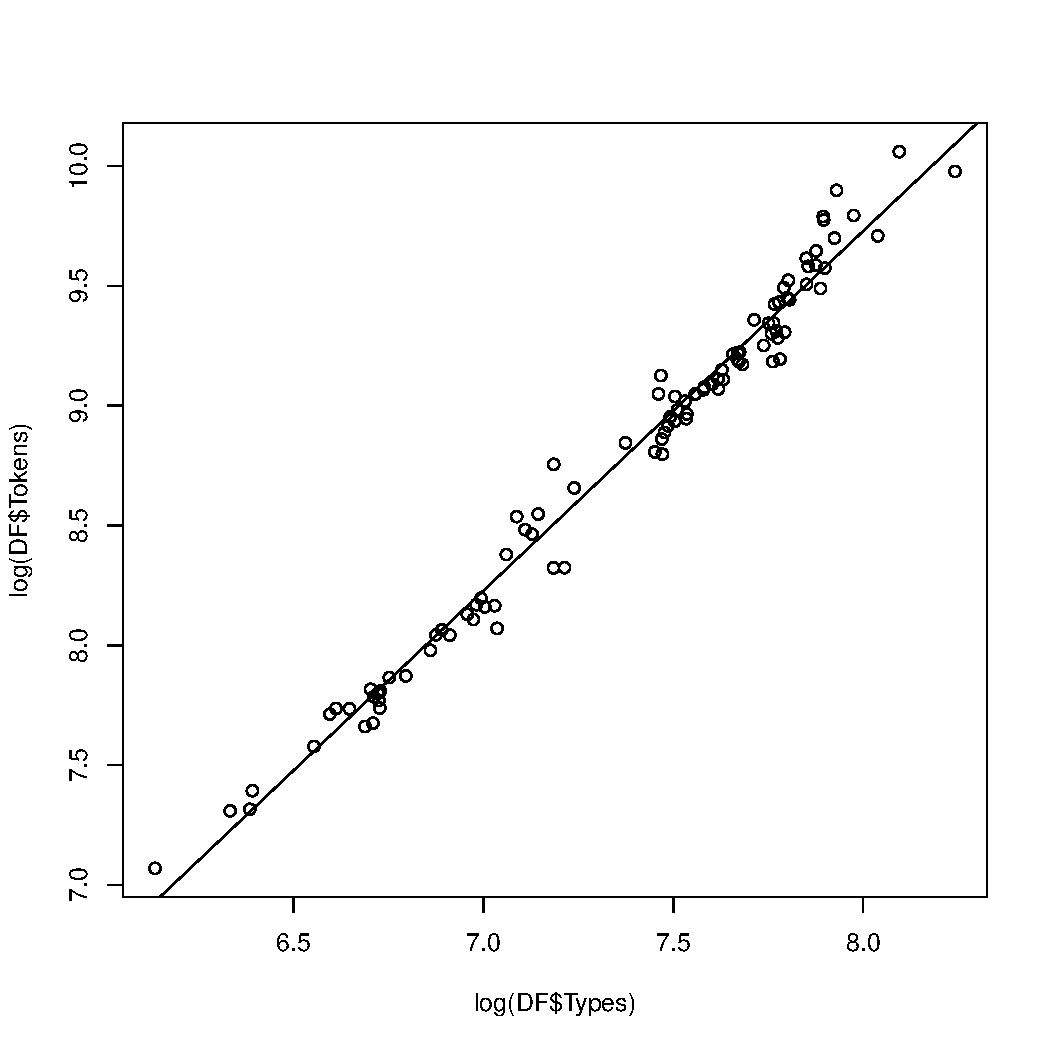
\includegraphics[scale=0.4]{figures/knitr-backupsotuillus-1.pdf}
\end{center}
\end{frame}
%%%%%%%%%%%%%%%%%%%%%%%%%%%%%%%%%%%%%%%%%%%%%%%%%%%%%%%%%%%%%%%%%%%%%%%%%

%%%%%%%%%%%%%%%%%%%%%%%%%%%%%%%%%%%%%%%%%%%%%%%%%%%%%%%%%%
\begin{frame}[fragile]{Illustration of Heap's Law in State of Union speeches}

\begin{knitrout}\tiny
\definecolor{shadecolor}{rgb}{0.969, 0.969, 0.969}\color{fgcolor}\begin{kframe}
\begin{alltt}
\hlkwd{summary}\hlstd{(}\hlkwd{lm}\hlstd{(}\hlkwd{log}\hlstd{(DF}\hlopt{$}\hlstd{Tokens)} \hlopt{~} \hlkwd{log}\hlstd{(DF}\hlopt{$}\hlstd{Types)))}
\end{alltt}
\begin{verbatim}
## 
## Call:
## lm(formula = log(DF$Tokens) ~ log(DF$Types))
## 
## Residuals:
##     Min      1Q  Median      3Q     Max 
## -0.2245 -0.0664 -0.0120  0.0603  0.2751 
## 
## Coefficients:
##               Estimate Std. Error t value Pr(>|t|)    
## (Intercept)    -2.2803     0.1569   -14.5   <2e-16 ***
## log(DF$Types)   1.5011     0.0212    70.7   <2e-16 ***
## ---
## Signif. codes:  0 '***' 0.001 '**' 0.01 '*' 0.05 '.' 0.1 ' ' 1
## 
## Residual standard error: 0.1 on 98 degrees of freedom
## Multiple R-squared:  0.981,	Adjusted R-squared:  0.981 
## F-statistic: 5e+03 on 1 and 98 DF,  p-value: <2e-16
\end{verbatim}
\end{kframe}
\end{knitrout}

For larger corpora, the coefficient is typically smaller. Stemming and further tokenization typically lowers the vocabulary space.

\end{frame}
%%%%%%%%%%%%%%%%%%%%%%%%%%%%%%%%%%%%%%%%%%%%%%%%%%%%%%%%%%%%%%%%%%%%%%%%%



%%%%%%%%%%%%%%%%%%%%%%%%%%%%%%%%%%%%%%%%%%%%%%%%%%%%%%%%%%
\begin{frame}[fragile]{Zipf's Law}
Zipf's Law is a law about the frequency distribution of words \emph{within a document}. 

Zipf's Law states that s frequency of any word is inversely proportional to its rank in the frequency table.\\

Formally: Word frequency

$$f = \frac{a}{r^b}$$

where $r$ is the rank in the (empirical) word frequency distribution. Again, logging

$$\log(f) = \log(a) - b \log(r)$$

\end{frame}
%%%%%%%%%%%%%%%%%%%%%%%%%%%%%%%%%%%%%%%%%%%%%%%%%%%%%%%%%%%%%%%%%%%%%%%%%


%%%%%%%%%%%%%%%%%%%%%%%%%%%%%%%%%%%%%%%%%%%%%%%%%%%%%%%%%%
\begin{frame}[fragile]{Illustration of Zipf's Law}
\begin{knitrout}\tiny
\definecolor{shadecolor}{rgb}{0.969, 0.969, 0.969}\color{fgcolor}\begin{kframe}
\begin{alltt}
\hlstd{OBAMA}\hlkwb{<-}\hlkwd{subset}\hlstd{(SOTUCorpus, filename}\hlopt{==}\hlstr{"su2012.txt"}\hlstd{)}
\hlstd{TOK}\hlkwb{<-}\hlkwd{tokenize}\hlstd{(OBAMA,} \hlkwc{removePunct}\hlstd{=}\hlnum{TRUE}\hlstd{)}
\hlstd{TOK}\hlkwb{<-}\hlkwd{data.table}\hlstd{(}\hlkwc{token}\hlstd{=}\hlkwd{tolower}\hlstd{(}\hlkwd{unlist}\hlstd{(TOK)))}
\hlstd{TOK}\hlkwb{<-}\hlstd{TOK[, .N,} \hlkwc{by}\hlstd{=token][}\hlkwd{order}\hlstd{(N,} \hlkwc{decreasing}\hlstd{=}\hlnum{TRUE}\hlstd{)]}
\hlstd{TOK[}\hlnum{1}\hlopt{:}\hlnum{20}\hlstd{]}
\end{alltt}
\begin{verbatim}
##     token   N
##  1:   the 294
##  2:    to 230
##  3:   and 204
##  4:    of 170
##  5:     a 160
##  6:  that 144
##  7:    in 108
##  8:   our  84
##  9:    we  84
## 10:   for  63
## 11:    is  59
## 12:  will  57
## 13:  this  52
## 14:    on  51
## 15:     i  50
## 16:    it  48
## 17:  with  47
## 18:  from  47
## 19:  more  43
## 20:    as  39
\end{verbatim}
\begin{alltt}
\hlstd{TOK[,rank} \hlkwb{:=}\hlnum{1}\hlopt{:}\hlkwd{nrow}\hlstd{(TOK)]}
\end{alltt}
\end{kframe}
\end{knitrout}
\end{frame}
%%%%%%%%%%%%%%%%%%%%%%%%%%%%%%%%%%%%%%%%%%%%%%%%%%%%%%%%%%%%%%%%%%%%%%%%%



%%%%%%%%%%%%%%%%%%%%%%%%%%%%%%%%%%%%%%%%%%%%%%%%%%%%%%%%%%
\begin{frame}[fragile]{Illustration of Zipf's Law}
\begin{knitrout}\tiny
\definecolor{shadecolor}{rgb}{0.969, 0.969, 0.969}\color{fgcolor}\begin{kframe}
\begin{alltt}
\hlkwd{plot}\hlstd{(}\hlkwd{log}\hlstd{(TOK}\hlopt{$}\hlstd{N),}\hlkwd{log}\hlstd{(TOK}\hlopt{$}\hlstd{rank))}\hlopt{+}\hlkwd{abline}\hlstd{(}\hlkwd{lm}\hlstd{(}\hlkwd{log}\hlstd{(TOK}\hlopt{$}\hlstd{N)} \hlopt{~} \hlkwd{log}\hlstd{(TOK}\hlopt{$}\hlstd{rank)))}
\end{alltt}
\begin{verbatim}
## numeric(0)
\end{verbatim}
\end{kframe}

{\centering 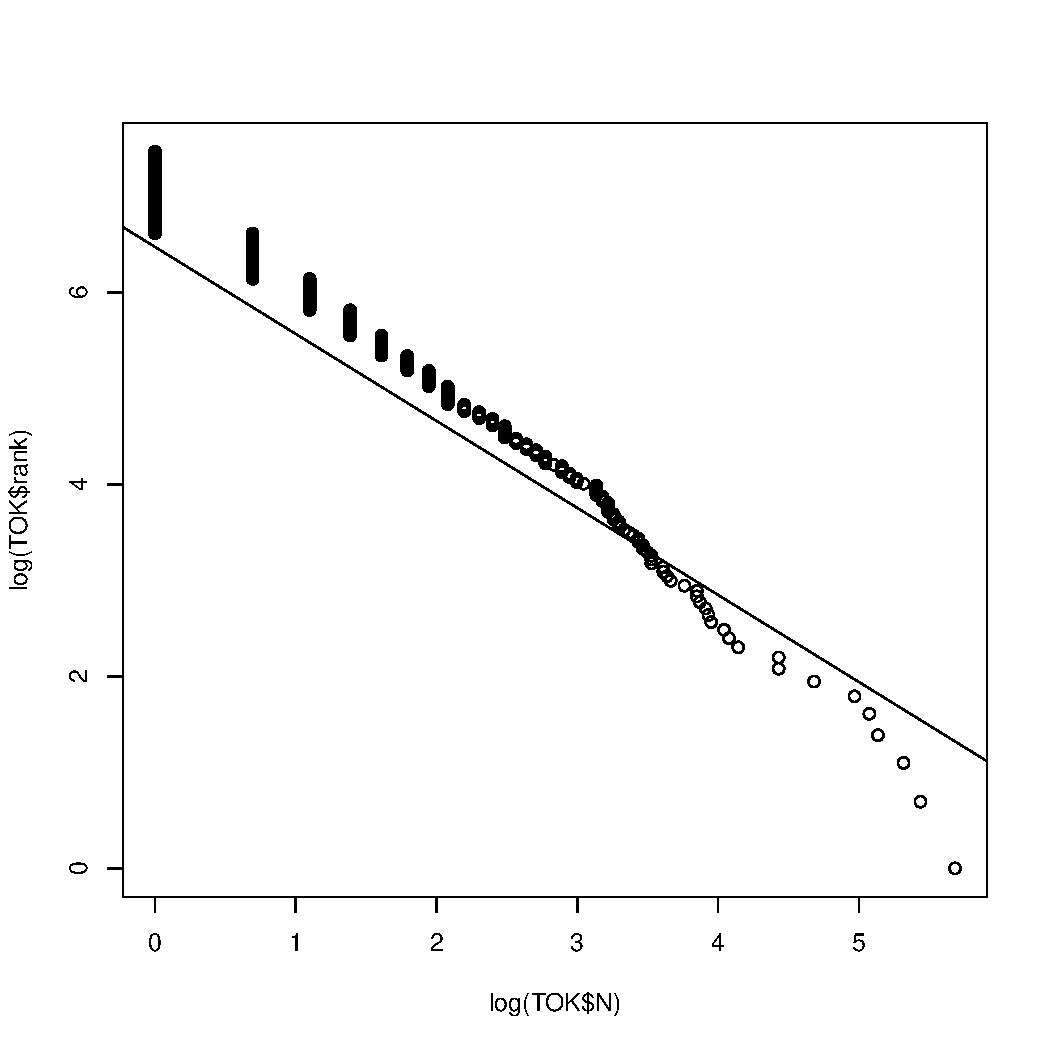
\includegraphics[width=3in]{figures/knitr-zipfsillustration2-1} 

}



\end{knitrout}
\end{frame}
%%%%%%%%%%%%%%%%%%%%%%%%%%%%%%%%%%%%%%%%%%%%%%%%%%%%%%%%%%%%%%%%%%%%%%%%%


%%%%%%%%%%%%%%%%%%%%%%%%%%%%%%%%%%%%%%%%%%%%%%%%%%%%%%%%%%
\begin{frame}[fragile]{Illustration of Zipf's Law}
\begin{knitrout}\tiny
\definecolor{shadecolor}{rgb}{0.969, 0.969, 0.969}\color{fgcolor}\begin{kframe}
\begin{alltt}
\hlkwd{summary}\hlstd{(}\hlkwd{lm}\hlstd{(}\hlkwd{log}\hlstd{(TOK}\hlopt{$}\hlstd{N)} \hlopt{~} \hlkwd{log}\hlstd{(TOK}\hlopt{$}\hlstd{rank)))}
\end{alltt}
\begin{verbatim}
## 
## Call:
## lm(formula = log(TOK$N) ~ log(TOK$rank))
## 
## Residuals:
##     Min      1Q  Median      3Q     Max 
## -0.7907 -0.1110  0.0411  0.1406  0.2938 
## 
## Coefficients:
##               Estimate Std. Error t value Pr(>|t|)    
## (Intercept)    6.47428    0.02937     220   <2e-16 ***
## log(TOK$rank) -0.90642    0.00449    -202   <2e-16 ***
## ---
## Signif. codes:  0 '***' 0.001 '**' 0.01 '*' 0.05 '.' 0.1 ' ' 1
## 
## Residual standard error: 0.186 on 1747 degrees of freedom
## Multiple R-squared:  0.959,	Adjusted R-squared:  0.959 
## F-statistic: 4.08e+04 on 1 and 1747 DF,  p-value: <2e-16
\end{verbatim}
\end{kframe}
\end{knitrout}
\end{frame}
%%%%%%%%%%%%%%%%%%%%%%%%%%%%%%%%%%%%%%%%%%%%%%%%%%%%%%%%%%%%%%%%%%%%%%%%%



%%%%%%%%%%%%%%%%%%%%%%%%%%%%%%%%%%%%%%%%%%%%%%%%%%%%%%%%%%
\begin{frame}[fragile]{Implications of Heap's and Zipf's Law}

\begin{itemize}

\item \emph{Heap's Law} and \emph{Zipf's Law} imply that data matrices constructed from text data is very \emph{sparse}.

\item Sparsity implies that there would be many zeroes.

\item Most data processing steps for text data involve \emph{densifying} the word frequency distribution. 

\item We next discuss a range of steps commonly used to densify.
\end{itemize}


\end{frame}
%%%%%%%%%%%%%%%%%%%%%%%%%%%%%%%%%%%%%%%%%%%%%%%%%%%%%%%%%%%%%%%%%%%%%%%%%



%%%%%%%%%%%%%%%%%%%%%%%%%%%%%%%%%%%%%%%%%%%%%%%%%%%%%%%%%%
\begin{frame}[fragile]{Word Tokenization and Normalization}

\begin{itemize}

\item \textbf{Tokenization} - task of segmenting running text into words.
\begin{itemize}

\item Plain vanilla approaches would just \code{str\_split(text," ")} - splitting by white spaces. 

\item More sophisticated methods apply \emph{locale} (language) specific algorithms.

\end{itemize}

\item \textbf{Normalization}- task of putting words/tokens into a standardized format.

\begin{itemize}
\item For example \code{we're} to \code{we are}.

\item Casefolding of tokens (lower-case or upper case)

\end{itemize}
\end{itemize}

\end{frame}
%%%%%%%%%%%%%%%%%%%%%%%%%%%%%%%%%%%%%%%%%%%%%%%%%%%%%%%%%%%%%%%%%%%%%%%%%


%%%%%%%%%%%%%%%%%%%%%%%%%%%%%%%%%%%%%%%%%%%%%%%%%%%%%%%%%%
\begin{frame}[fragile]{\code{quanteda} tokenization routine}
We have already used the functionality in a few illustrations, but lets systematically introduce it here.

\begin{knitrout}\tiny
\definecolor{shadecolor}{rgb}{0.969, 0.969, 0.969}\color{fgcolor}\begin{kframe}
\begin{alltt}
\hlkwd{tokenize}\hlstd{(x,} \hlkwc{what} \hlstd{=} \hlkwd{c}\hlstd{(}\hlstr{"word"}\hlstd{,} \hlstr{"sentence"}\hlstd{,} \hlstr{"character"}\hlstd{,}
  \hlstr{"fastestword"}\hlstd{,} \hlstr{"fasterword"}\hlstd{),} \hlkwc{removeNumbers} \hlstd{=} \hlnum{FALSE}\hlstd{,} \hlkwc{removePunct} \hlstd{=} \hlnum{FALSE}\hlstd{,}
  \hlkwc{removeSymbols} \hlstd{=} \hlnum{FALSE}\hlstd{,} \hlkwc{removeSeparators} \hlstd{=} \hlnum{TRUE}\hlstd{,} \hlkwc{removeTwitter} \hlstd{=} \hlnum{FALSE}\hlstd{,}
  \hlkwc{removeHyphens} \hlstd{=} \hlnum{FALSE}\hlstd{,} \hlkwc{removeURL} \hlstd{=} \hlnum{FALSE}\hlstd{,} \hlkwc{ngrams} \hlstd{=} \hlnum{1L}\hlstd{,} \hlkwc{skip} \hlstd{=} \hlnum{0L}\hlstd{,}
  \hlkwc{concatenator} \hlstd{=} \hlstr{"_"}\hlstd{,} \hlkwc{simplify} \hlstd{=} \hlnum{FALSE}\hlstd{,} \hlkwc{verbose} \hlstd{=} \hlnum{FALSE}\hlstd{, ...)}
\end{alltt}
\end{kframe}
\end{knitrout}

Tokenization function allows separation of words, sentences and individual characters from a character vector $x$ or a corpus object.  
\begin{center}
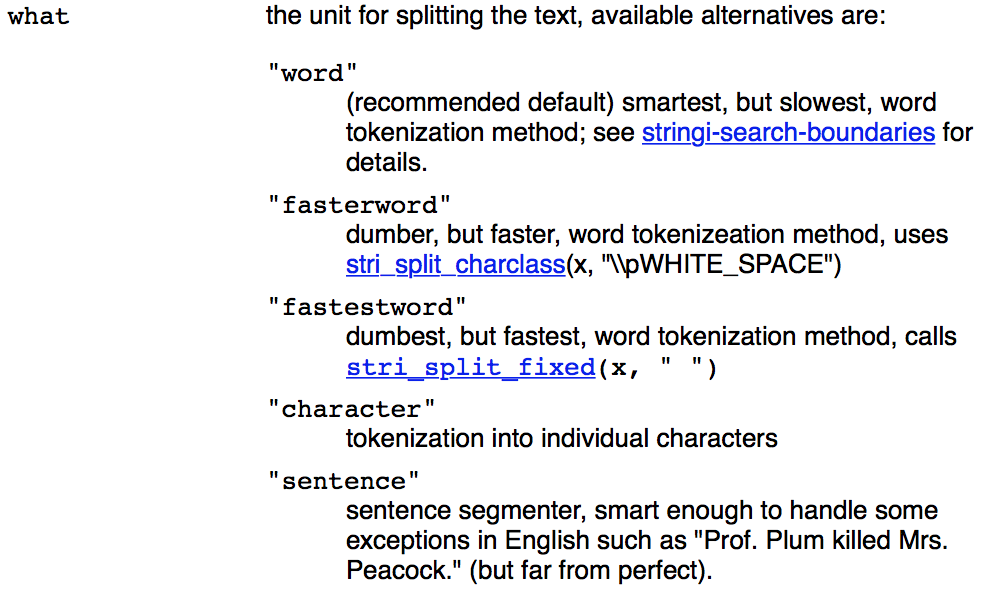
\includegraphics[scale=0.4]{figures/tokenizer-options.png}
\end{center}
\end{frame}
%%%%%%%%%%%%%%%%%%%%%%%%%%%%%%%%%%%%%%%%%%%%%%%%%%%%%%%%%%%%%%%%%%%%%%%%%



%%%%%%%%%%%%%%%%%%%%%%%%%%%%%%%%%%%%%%%%%%%%%%%%%%%%%%%%%%
\begin{frame}[fragile]{\code{quanteda} tokenization routine}
\begin{itemize}

\item Dumb tokenization approach works reasonably well for languages based on latin alphabet. 
\item You may end up tokenizing features that you do not really want to separate, like \emph{Named Entities} - \code{New York} (next week we will work on detecting such n-grams)

\item Works poorly for languages that do not use white space character for separation (e.g. Chinese)

\item \code{word} option uses the \code{BreakIterator} algorithm that implements the \emph{Unicode Text Segmentation} standard

\item Words boundaries are identified according to the rules in \url{http://www.unicode.org/reports/tr29/#Word_Boundaries}, supplemented by a word dictionary for text in Chinese, Japanese, Thai or Khmer. The rules used for locating word breaks take into account the alphabets and conventions used by different languages.

\end{itemize}
\end{frame}
%%%%%%%%%%%%%%%%%%%%%%%%%%%%%%%%%%%%%%%%%%%%%%%%%%%%%%%%%%%%%%%%%%%%%%%%%


%%%%%%%%%%%%%%%%%%%%%%%%%%%%%%%%%%%%%%%%%%%%%%%%%%%%%%%%%%
\begin{frame}[fragile]{\code{quanteda} tokenization routine}
Lets look at impact of the three alternative word tokenization methods for Obama's speeches.
\begin{knitrout}\tiny
\definecolor{shadecolor}{rgb}{0.969, 0.969, 0.969}\color{fgcolor}\begin{kframe}
\begin{alltt}
\hlkwa{for}\hlstd{(i} \hlkwa{in} \hlkwd{c}\hlstd{(}\hlstr{"word"}\hlstd{,} \hlstr{"fastestword"}\hlstd{,} \hlstr{"fasterword"}\hlstd{)) \{}
  \hlstd{TOK}\hlkwb{<-}\hlkwd{data.table}\hlstd{(}\hlkwc{tok}\hlstd{=}\hlkwd{unlist}\hlstd{(}\hlkwd{tokenize}\hlstd{(OBAMA,} \hlkwc{what}\hlstd{=i,} \hlkwc{removePunct}\hlstd{=}\hlnum{TRUE}\hlstd{)))[ ,.N,} \hlkwc{by}\hlstd{=tok][}\hlkwd{order}\hlstd{(N,} \hlkwc{decreasing}\hlstd{=}\hlnum{TRUE}\hlstd{)]}
  \hlstd{TOK[, rid} \hlkwb{:=} \hlnum{1}\hlopt{:}\hlkwd{nrow}\hlstd{(TOK)]}
\hlkwd{plot}\hlstd{(}\hlkwd{hist}\hlstd{(}\hlkwd{log}\hlstd{(TOK}\hlopt{$}\hlstd{N)),} \hlkwc{main}\hlstd{=i)}
\hlstd{\}}
\end{alltt}
\end{kframe}
\end{knitrout}
\begin{figure}[h!]
\begin{center}$
\begin{array}{ccc}
 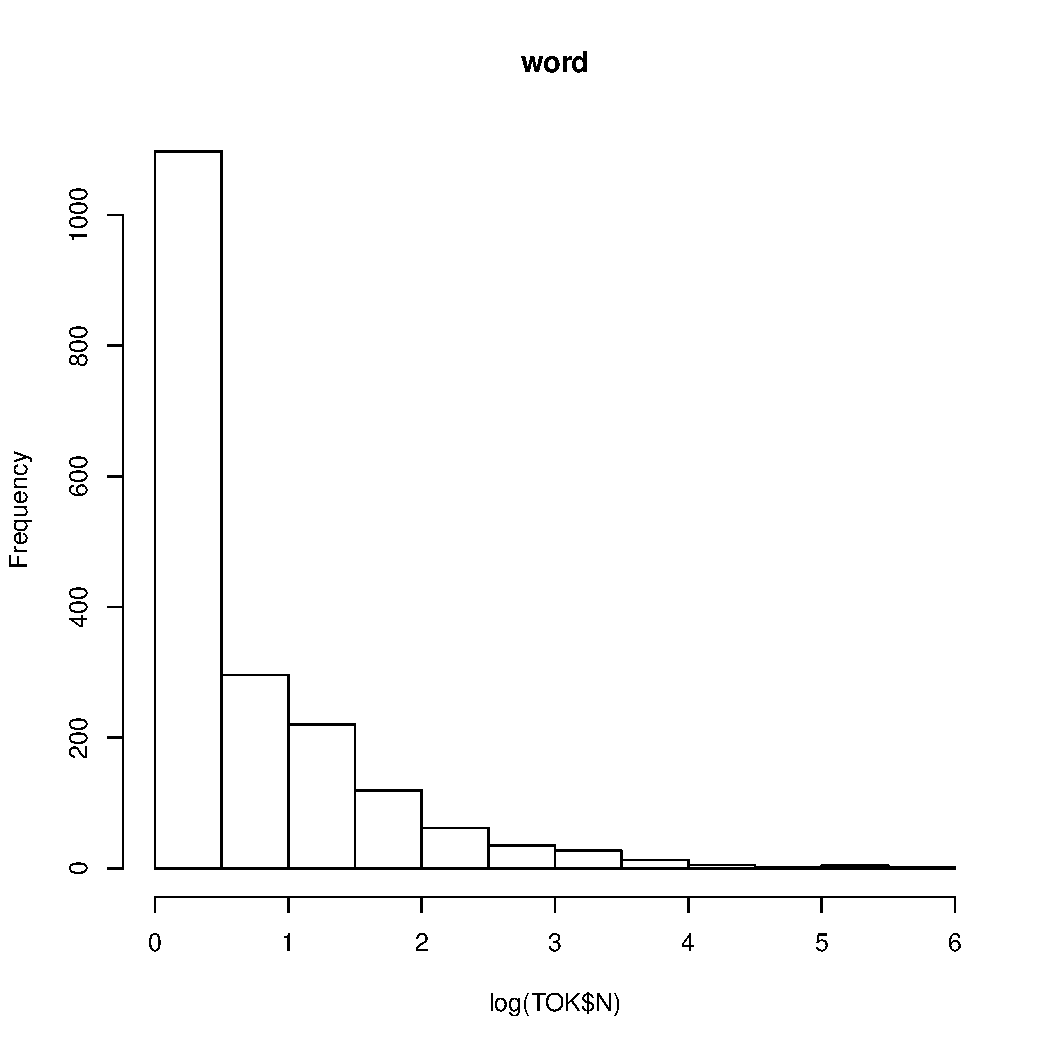
\includegraphics[scale=.2]{figures/knitr-tokenizefunctionmethods-2.pdf}&  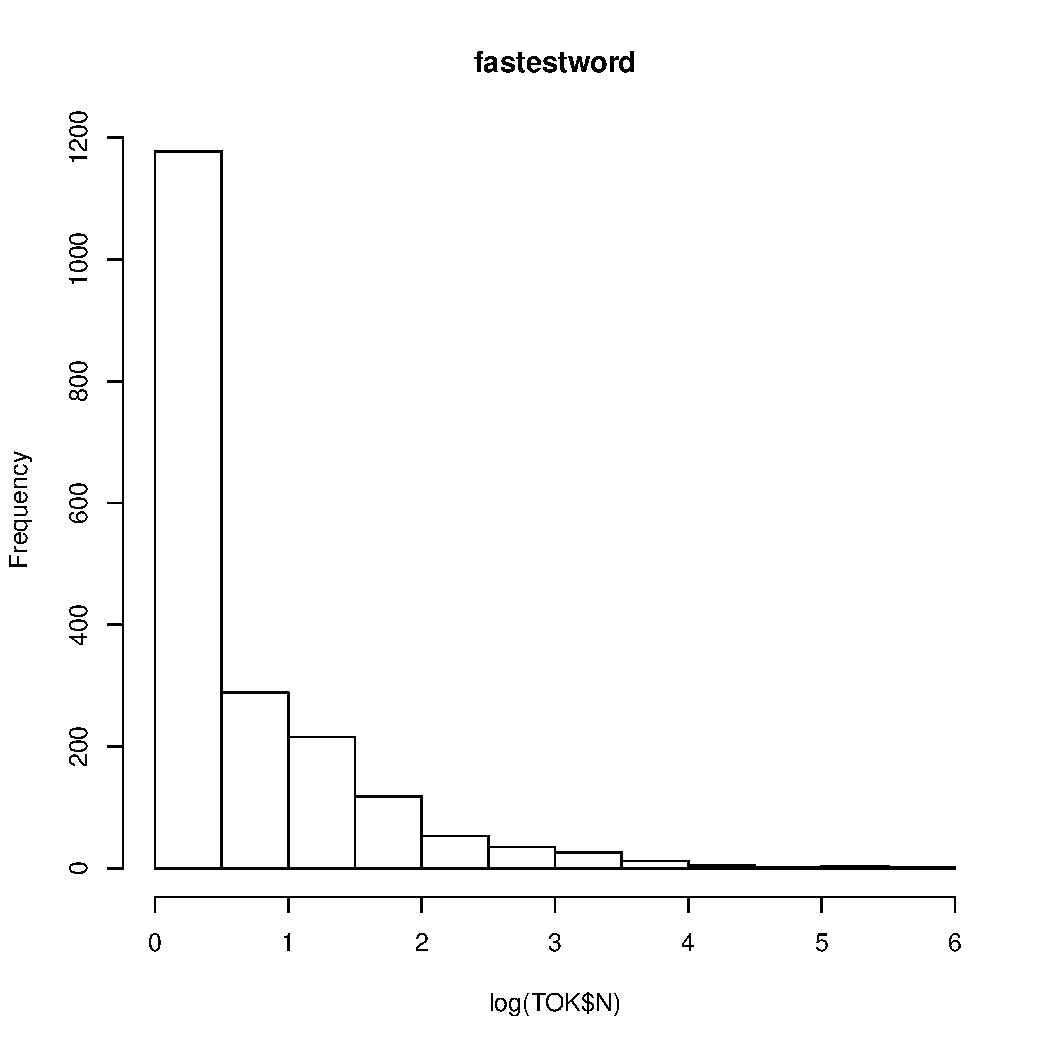
\includegraphics[scale=.2]{figures/knitr-tokenizefunctionmethods-4.pdf}& 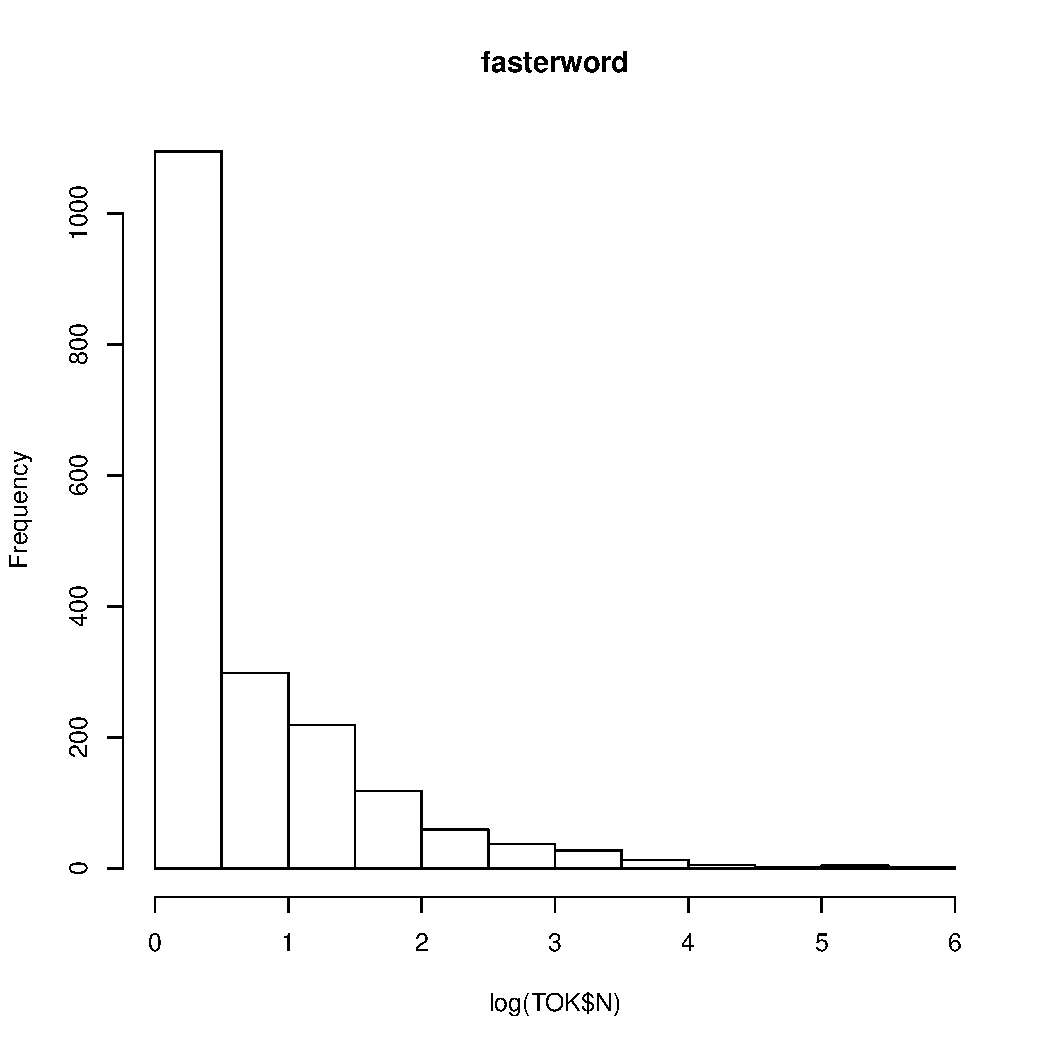
\includegraphics[scale=.2]{figures/knitr-tokenizefunctionmethods-6.pdf}
\end{array}$
\end{center}
\end{figure}
We \emph{may} want to shift more mass to the right (higher counts). Little effect of densification of distribution of token counts using different methods.
\end{frame}
%%%%%%%%%%%%%%%%%%%%%%%%%%%%%%%%%%%%%%%%%%%%%%%%%%%%%%%%%%%%%%%%%%%%%%%%%


%%%%%%%%%%%%%%%%%%%%%%%%%%%%%%%%%%%%%%%%%%%%%%%%%%%%%%%%%%
\begin{frame}[fragile]{\code{quanteda} tokenization routine}
\begin{itemize}
\item Depending on the application or which the data is prepared, it may make sense to normalize text by lowercaseing it, removing punctuation (as we have done already).

\item This may introduce \emph{noise} or inaccuracies, but its important to bear in mind what is the goal of the application.

\item in $R$, lowercasing is achieved with the function \code{tolower()}.

\end{itemize}

\end{frame}
%%%%%%%%%%%%%%%%%%%%%%%%%%%%%%%%%%%%%%%%%%%%%%%%%%%%%%%%%%%%%%%%%%%%%%%%%


%%%%%%%%%%%%%%%%%%%%%%%%%%%%%%%%%%%%%%%%%%%%%%%%%%%%%%%%%%
\begin{frame}[fragile]{Lemmatization and Stemming}

Sparsity is a central issue as it blows up the underlying data matrices we work with.  There are a range of methods to select features and densify resulting data matrices.

\begin{Description}

\item[document frequency] cutoffs around how many documents does a term appear. 

\item[term frequency] cutoffs around how often a term appears in a corpus

\item[lemmatization] densification based on identified linguistic roots, disregarding the underlying parts of speech (verbs and adjective)

\item[deliberate disregard] exclude a range of stop words: words that do not provide independent substantive content

\item[purposive selection] use of dictionaries of words or phrases, possible identified from the underlying data (like collocations) or identified as having ``predictive content'' along dimension of interest.

\item[declared equivalency class] work of synonyms and map word (stems) to their underlying synonym

\end{Description}

We will discuss these in the next set of slides...
\end{frame}
%%%%%%%%%%%%%%%%%%%%%%%%%%%%%%%%%%%%%%%%%%%%%%%%%%%%%%%%%%%%%%%%%%%%%%%%%



%%%%%%%%%%%%%%%%%%%%%%%%%%%%%%%%%%%%%%%%%%%%%%%%%%%%%%%%%%
\begin{frame}[fragile]{Lemmatization and Stemming}

Lemmatization is the task of determining that two words have the same linguisting root.

\begin{itemize}

\item \code{am, are, is} have the same root being \code{be}

\item Plural's for nouns, in English usually identified by an added \code{s} share the same root.

\item Other gramatic constructs, like \emph{superlatives}...

\end{itemize}

The most common approach for English is to work with the \emph{Porter stemmer}, which simply chops off affixes. More complex methods use look up tables or augment process with information on the Part of Speech.

\end{frame}
%%%%%%%%%%%%%%%%%%%%%%%%%%%%%%%%%%%%%%%%%%%%%%%%%%%%%%%%%%%%%%%%%%%%%%%%%


%%%%%%%%%%%%%%%%%%%%%%%%%%%%%%%%%%%%%%%%%%%%%%%%%%%%%%%%%%
\begin{frame}[fragile]{Porter Stemmer}

\begin{itemize}

\item Algorithm dates from 1980
\item Still the default ``go-to'' stemmer as it provides a good  trade-off between speed, readability, and accuracy

\item Stems using a set of rules, or transformations, applied in a succession of steps

\item In total there are about 60 rules in 6 steps that are applied iteratively
\end{itemize}

The sequence of steps can be summarized as follows:
\begin{enumerate}
\item Get rid of plurals and \code{-ed} or \code{-ing} suffixes
\item Turns terminal \code{y} to \code{i} when there is another vowel in the stem

\item Maps double suffixes to single ones: \code{-ization}, \code{-ational}, etc.

\item Deals with suffixes, \code{-full}, \code{-ness} etc.

\item Takes off \code{-ant}, \code{-ence}, etc.

\item Removes a final \code{-e} 

\end{enumerate}
\end{frame}
%%%%%%%%%%%%%%%%%%%%%%%%%%%%%%%%%%%%%%%%%%%%%%%%%%%%%%%%%%%%%%%%%%%%%%%%%


%%%%%%%%%%%%%%%%%%%%%%%%%%%%%%%%%%%%%%%%%%%%%%%%%%%%%%%%%%
\begin{frame}[fragile]{Porter Stemmer Examples}

\begin{enumerate}
\item Get rid of plurals and \code{-ed} or \code{-ing} suffixes
\item Turns terminal \code{y} to \code{i} when there is another vowel in the stem

\item Maps double suffixes to single ones: \code{-ization}, \code{-ational}, etc.

\item Deals with suffixes, \code{-full}, \code{-ness} etc.

\item Takes off \code{-ant}, \code{-ence}, etc.

\item Removes a final \code{-e} 

\end{enumerate}

Semantically $\rightarrow$ semantically $\rightarrow$ semanticalli $\rightarrow$ semantical  $\rightarrow$ semantic $\rightarrow$ semant $\rightarrow$ semant. \smallskip


Destructiveness $\rightarrow$ destructiveness $\rightarrow$ destructiveness $\rightarrow$ destructive $\rightarrow$ destructive $\rightarrow$ destruct $\rightarrow$ destruct\smallskip

Recognizing $\rightarrow$ recognize $\rightarrow$ recognize $\rightarrow$ recognize $\rightarrow$ recognize $\rightarrow$ recognize $\rightarrow$ recognize

Online illustration: \url{http://9ol.es/porter_js_demo.html}

\end{frame}
%%%%%%%%%%%%%%%%%%%%%%%%%%%%%%%%%%%%%%%%%%%%%%%%%%%%%%%%%%%%%%%%%%%%%%%%%


%%%%%%%%%%%%%%%%%%%%%%%%%%%%%%%%%%%%%%%%%%%%%%%%%%%%%%%%%%
\begin{frame}[fragile]{$R$ implementation}

Most implementaiton of Porter stemmer used in $R$ are actually coded in $C$, as $C++$ is much faster in processing.

\begin{knitrout}\tiny
\definecolor{shadecolor}{rgb}{0.969, 0.969, 0.969}\color{fgcolor}\begin{kframe}
\begin{alltt}
\hlkwd{library}\hlstd{(}\hlstr{"SnowballC"}\hlstd{)}

\hlkwd{wordStem}\hlstd{(}\hlstr{"Amazing"}\hlstd{)}
\end{alltt}
\begin{verbatim}
## [1] "Amaze"
\end{verbatim}
\begin{alltt}
\hlcom{#multiple languages are supported}
\hlkwd{getStemLanguages}\hlstd{()}
\end{alltt}
\begin{verbatim}
##  [1] "danish"     "dutch"      "english"    "finnish"    "french"     "german"    
##  [7] "hungarian"  "italian"    "norwegian"  "porter"     "portuguese" "romanian"  
## [13] "russian"    "spanish"    "swedish"    "turkish"
\end{verbatim}
\begin{alltt}
\hlkwd{wordStem}\hlstd{(}\hlstr{"Liebschaften"}\hlstd{,} \hlkwc{language}\hlstd{=}\hlstr{"de"}\hlstd{)}
\end{alltt}
\begin{verbatim}
## [1] "Liebschaft"
\end{verbatim}
\begin{alltt}
\hlkwd{wordStem}\hlstd{(}\hlstr{"amaren"}\hlstd{,} \hlkwc{language}\hlstd{=}\hlstr{"es"}\hlstd{)}
\end{alltt}
\begin{verbatim}
## [1] "amar"
\end{verbatim}
\begin{alltt}
\hlcom{#densification?}
\hlstd{TOK[, stemmed} \hlkwb{:=} \hlkwd{wordStem}\hlstd{(tok)]}
\hlkwd{nrow}\hlstd{(TOK)}
\end{alltt}
\begin{verbatim}
## [1] 1877
\end{verbatim}
\begin{alltt}
\hlkwd{summary}\hlstd{(TOK}\hlopt{$}\hlstd{N)}
\end{alltt}
\begin{verbatim}
##    Min. 1st Qu.  Median    Mean 3rd Qu.    Max. 
##     1.0     1.0     1.0     3.7     3.0   278.0
\end{verbatim}
\begin{alltt}
\hlstd{STEM}\hlkwb{<-}\hlstd{TOK[,} \hlkwd{sum}\hlstd{(N),}\hlkwc{by}\hlstd{=stemmed]}
\hlkwd{plot}\hlstd{(}\hlkwd{hist}\hlstd{(}\hlkwd{log}\hlstd{(STEM}\hlopt{$}\hlstd{V1)))}
\end{alltt}
\end{kframe}
\end{knitrout}


\end{frame}
%%%%%%%%%%%%%%%%%%%%%%%%%%%%%%%%%%%%%%%%%%%%%%%%%%%%%%%%%%%%%%%%%%%%%%%%%



%%%%%%%%%%%%%%%%%%%%%%%%%%%%%%%%%%%%%%%%%%%%%%%%%%%%%%%%%%
\begin{frame}[fragile]{Stemming reduces dimensionality}

\begin{center}
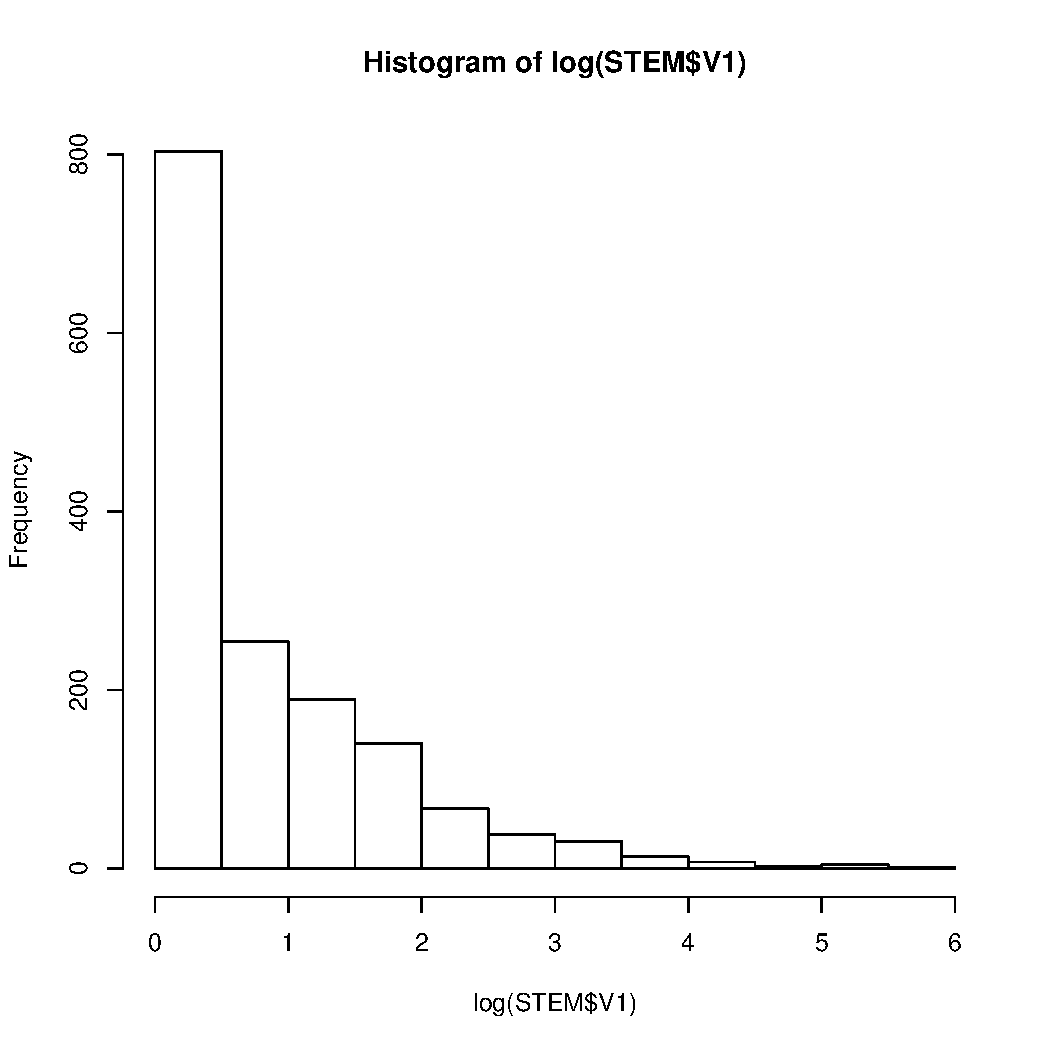
\includegraphics[scale=0.38]{figures/knitr-snowball-1.pdf}
\end{center}

Mass is shifted to the right, away from words occuring just once.
\end{frame}
%%%%%%%%%%%%%%%%%%%%%%%%%%%%%%%%%%%%%%%%%%%%%%%%%%%%%%%%%%%%%%%%%%%%%%%%%


%%%%%%%%%%%%%%%%%%%%%%%%%%%%%%%%%%%%%%%%%%%%%%%%%%%%%%%%%%
\begin{frame}[fragile]{Stemming Issues}

Stemming is an approximation to the Lemmatization task which generally provides for a good trade-off between accuracy and speed. Most are stimple rule based algorithms.

\begin{itemize}

\item Stemmers are rudimentary approach to morphological analysis

\item No word sense disambiguation (``Police`` vs ``policing``)

\item No Part of Speech disambiguation (``Policing`` could be noun or verb, but ``hitting`` could only be verb)

\item However other approaches to lemmatization in practice does not do
much better. 

\end{itemize}

We just briefly introduce an alternative $R$ package that implements a morphological approach.
\end{frame}
%%%%%%%%%%%%%%%%%%%%%%%%%%%%%%%%%%%%%%%%%%%%%%%%%%%%%%%%%%%%%%%%%%%%%%%%%


%%%%%%%%%%%%%%%%%%%%%%%%%%%%%%%%%%%%%%%%%%%%%%%%%%%%%%%%%%
\begin{frame}[fragile]{\code{hunspell} package}

\begin{itemize}

\item \code{hunspell} is actually the spell checker used in Google Chrome, which is also used by other proprietary software packages.

\item Has a significant capacities to identify lemmas of words using a dictionary lookup approach.

\end{itemize}

\begin{knitrout}\tiny
\definecolor{shadecolor}{rgb}{0.969, 0.969, 0.969}\color{fgcolor}\begin{kframe}
\begin{alltt}
\hlstd{words} \hlkwb{<-} \hlkwd{c}\hlstd{(}\hlstr{"severing"}\hlstd{,} \hlstr{"several"}\hlstd{,} \hlstr{"ironic"}\hlstd{,} \hlstr{"iron"}\hlstd{,} \hlstr{"animal"}\hlstd{,} \hlstr{"animated"}\hlstd{)}
\hlkwd{wordStem}\hlstd{(words)}
\end{alltt}
\begin{verbatim}
## [1] "sever" "sever" "iron"  "iron"  "anim"  "anim"
\end{verbatim}
\begin{alltt}
\hlkwd{library}\hlstd{(hunspell)}
\hlcom{#hunspell_stem(words)}
\hlkwd{hunspell_analyze}\hlstd{(words)}
\end{alltt}
\begin{verbatim}
## [[1]]
## [1] " st:severing"   " st:sever fl:G"
## 
## [[2]]
## [1] " st:several"
## 
## [[3]]
## [1] " st:ironic"
## 
## [[4]]
## [1] " st:iron"
## 
## [[5]]
## [1] " st:animal"
## 
## [[6]]
## [1] " st:animated"     " st:animate fl:D"
\end{verbatim}
\end{kframe}
\end{knitrout}



\end{frame}
%%%%%%%%%%%%%%%%%%%%%%%%%%%%%%%%%%%%%%%%%%%%%%%%%%%%%%%%%%%%%%%%%%%%%%%%%



%%%%%%%%%%%%%%%%%%%%%%%%%%%%%%%%%%%%%%%%%%%%%%%%%%%%%%%%%%
\begin{frame}[fragile]{\code{stopwords}}

Stopwords are words that typically contain no informational content, they may be articles, prepositions, ...

\begin{knitrout}\tiny
\definecolor{shadecolor}{rgb}{0.969, 0.969, 0.969}\color{fgcolor}\begin{kframe}
\begin{alltt}
\hlkwd{stopwords}\hlstd{(}\hlstr{"english"}\hlstd{)[}\hlnum{1}\hlopt{:}\hlnum{20}\hlstd{]}
\end{alltt}
\begin{verbatim}
##  [1] "i"          "me"         "my"         "myself"     "we"         "our"       
##  [7] "ours"       "ourselves"  "you"        "your"       "yours"      "yourself"  
## [13] "yourselves" "he"         "him"        "his"        "himself"    "she"       
## [19] "her"        "hers"
\end{verbatim}
\begin{alltt}
\hlkwd{stopwords}\hlstd{(}\hlstr{"spanish"}\hlstd{)[}\hlnum{1}\hlopt{:}\hlnum{20}\hlstd{]}
\end{alltt}
\begin{verbatim}
##  [1] "de"   "la"   "que"  "el"   "en"   "y"    "a"    "los"  "del"  "se"   "las"  "por" 
## [13] "un"   "para" "con"  "no"   "una"  "su"   "al"   "lo"
\end{verbatim}
\begin{alltt}
\hlkwd{stopwords}\hlstd{(}\hlstr{"german"}\hlstd{)[}\hlnum{1}\hlopt{:}\hlnum{20}\hlstd{]}
\end{alltt}
\begin{verbatim}
##  [1] "aber"    "alle"    "allem"   "allen"   "aller"   "alles"   "als"     "also"   
##  [9] "am"      "an"      "ander"   "andere"  "anderem" "anderen" "anderer" "anderes"
## [17] "anderm"  "andern"  "anderr"  "anders"
\end{verbatim}
\end{kframe}
\end{knitrout}

Identifying words that can be removed as they are stopwords may use statistical methods, such as corpus dissimilarity, which we will introduce in the collocation detection lecture this week.

In \code{quanteda} you can remove features from a \code{tokenize}-object by applying the \code{removeFeatures(x, features)}, where \code{features} could be \code{stopwords("english")}.

\end{frame}
%%%%%%%%%%%%%%%%%%%%%%%%%%%%%%%%%%%%%%%%%%%%%%%%%%%%%%%%%%%%%%%%%%%%%%%%%


%%%%%%%%%%%%%%%%%%%%%%%%%%%%%%%%%%%%%%%%%%%%%%%%%%%%%%%%%%
\begin{frame}[fragile]{Wordnet based densification}
\begin{quote}
WordNet is a large lexical database of English. Nouns, verbs, adjectives and adverbs are grouped into sets of cognitive synonyms (synsets), each expressing a distinct concept. Synsets are interlinked by means of conceptual-semantic and lexical relations. 
\end{quote}

\begin{itemize}

\item Need to separately install wordnet, in Mac can be done quickly using homebrew. 
\code{brew install wordnet}

\item R-package called \code{wordnet}

\item On loading, need to set path to wordnet dictionary installation.

\item Available to browse on \url{http://wordnetweb.princeton.edu/perl/webwn?s=car}
\end{itemize}

\end{frame}
%%%%%%%%%%%%%%%%%%%%%%%%%%%%%%%%%%%%%%%%%%%%%%%%%%%%%%%%%%%%%%%%%%%%%%%%%


%%%%%%%%%%%%%%%%%%%%%%%%%%%%%%%%%%%%%%%%%%%%%%%%%%%%%%%%%%
\begin{frame}[fragile]{Wordnet based densification}
\begin{knitrout}\tiny
\definecolor{shadecolor}{rgb}{0.969, 0.969, 0.969}\color{fgcolor}\begin{kframe}
\begin{alltt}
\hlkwd{library}\hlstd{(wordnet)}
\hlcom{#set path to dictionary}
\hlkwd{setDict}\hlstd{(}\hlstr{"/usr/local/Cellar/wordnet/3.1/dict"}\hlstd{)}
\hlkwd{synonyms}\hlstd{(}\hlstr{"company"}\hlstd{,} \hlstr{"NOUN"}\hlstd{)}
\end{alltt}
\begin{verbatim}
## [1] "caller"         "companionship"  "company"        "fellowship"     "party"         
## [6] "ship's company" "society"        "troupe"
\end{verbatim}
\end{kframe}
\end{knitrout}
Could list word list (running part of speech tagging first) and then replace synonyms of most frequently appearing words to reduce the vocabulary.
\end{frame}
%%%%%%%%%%%%%%%%%%%%%%%%%%%%%%%%%%%%%%%%%%%%%%%%%%%%%%%%%%%%%%%%%%%%%%%%%



%%%%%%%%%%%%%%%%%%%%%%%%%%%%%%%%%%%%%%%%%%%%%%%%%%%%%%%%%%
\begin{frame}[fragile]{Minimum Edit Distances}

A lot of NLP work consists of identifying which texts are similar to others. We will illustrate this later, when we turn to a \emph{bag of words} language model that allows simple \emph{vector based} comparisons of text.\smallskip

We introduce the idea of computing string similarity introducing the idea of Edit Distance.\smallskip

Levenshtein distance between two words is the minimum number of single-character edits (i.e. insertions, deletions or substitutions) required to change one word into the other.
I will show an application from my research.\smallskip

This is extremely useful when working with (messy) data - such as OCRed documents, where you need to get standardize and get rid of non-systematic typos. \smallskip


\end{frame}
%%%%%%%%%%%%%%%%%%%%%%%%%%%%%%%%%%%%%%%%%%%%%%%%%%%%%%%%%%%%%%%%%%%%%%%%%


%%%%%%%%%%%%%%%%%%%%%%%%%%%%%%%%%%%%%%%%%%%%%%%%%%%%%%%%%%
\begin{frame}[fragile]{Levenshtein Distance}

\begin{itemize}

\item Levenshtein distance assumes a cost of deletion/ insertion of a character to be 1.

\item Assumes a cost of substition of character of 1 (sometimes 2).

\item So the Levenshtein distance between \code{car} and \code{can} is equal to 1.

\item Unit cost allows express adjustments needed relative to string length.

\item Levenshtein computation uses \textbf{dynamic programming} and is thus very fast.

\begin{quote}
dynamic programming (also known as dynamic optimization) is a method for solving a complex problem by breaking it down into a collection of simpler subproblems, solving each of those subproblems
\end{quote}

\end{itemize}
\end{frame}
%%%%%%%%%%%%%%%%%%%%%%%%%%%%%%%%%%%%%%%%%%%%%%%%%%%%%%%%%%%%%%%%%%%%%%%%%


%%%%%%%%%%%%%%%%%%%%%%%%%%
\begin{frame}[fragile]{Minimum Edit Distances}
Suppose you have two strings $s$ and $t$ of length $n$ and $m$.

Below provides the algorithm
\begin{table}
\scalebox{0.7}{
\begin{tabular}{ll}
\toprule
Step & Description \\
\midrule
1 & Set n to be the length of a. \\
 & Set m to be the length of b. \\
 & If $n = 0$, return m and exit. \\
 & If $m = 0$, return n and exit. \\
 & Construct a matrix containing $0..m$ rows and $0..n$ columns. \\
2 & Initialize the first row to $0..n$. \\
 & Initialize the first column to 0..m. \\
3 & Examine each character of a (i from 1 to n). \\
4 & Examine each character of b (j from 1 to m). \\
5 & If $a[i]$ equals $b[j]$, the cost is 0. \\
 & If $a[i]$ doesn't equal $b[j]$, the cost is 1. \\
6 & Set cell d[i,j] of the matrix equal to the minimum of: \\
 & a. The cell immediately above plus 1: $d[i-1,j] + 1$. \\
 & b. The cell immediately to the left plus 1: $d[i,j-1] + 1$. \\
 & c. The cell diagonally above and to the left plus the cost: $d[i-1,j-1] + cost$. \\
7 & After the iteration steps (3, 4, 5, 6) are complete, the distance is found in cell $d[n,m]$. \\

\bottomrule
\end{tabular}
}
\end{table}

\end{frame}
%%%%%%%%%%%%%%%%%%%%%%%%%%%%%%%%%%%%%%%%%%%%%%%%%%%%%%%%%%%%%%%%%%%%%%%%%



%%%%%%%%%%%%%%%%%%%%%%%%%%%%%%%%%%%%%%%%%%%%%%%%%%%%%%%%%%
\begin{frame}[fragile]{Levenshtein Distance}

Formally, Levenshtein Distance is computed as

$$ \qquad\operatorname{lev}_{a,b}(i,j) = min \begin{cases}
          \operatorname{lev}_{a,b}(i-1,j) + 1 \\
          \operatorname{lev}_{a,b}(i,j-1) + 1 \\
          \operatorname{lev}_{a,b}(i-1,j-1) + 1_{(a_i \neq b_j)}
       \end{cases} $$
       
       
\end{frame}
%%%%%%%%%%%%%%%%%%%%%%%%%%%%%%%%%%%%%%%%%%%%%%%%%%%%%%%%%%%%%%%%%%%%%%%%%




%%%%%%%%%%%%%%%%%%%%%%%%%%%%%%%%%%%%%%%%%%%%%%%%%%%%%%%%%%
\begin{frame}[fragile]{An Illustration}
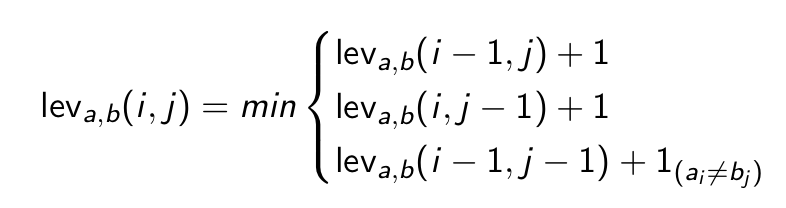
\includegraphics[scale=.35]{figures/lev-computation.png}

\textbf{Initialization} Step 1 and 2

\begin{table}
\begin{center}
\begin{tabular}{llllllllllll}
\toprule
 &  & e & x & e & c & u & t & i & o & n \\
\midrule
 & 0 & 1 & 2 & 3 & 4 & 5 & 6 & 7 & 8 & 9 \\
i & 1 \\
n & 2  \\
t & 3 \\
e & 4 \\
n & 5 \\
t & 6 \\
i & 7 \\
o & 8 \\
n & 9 &  &  &  &  &  &  &  &  &  \\
\bottomrule
\end{tabular}
\end{center}
\end{table}



\end{frame}
%%%%%%%%%%%%%%%%%%%%%%%%%%%%%%%%%%%%%%%%%%%%%%%%%%%%%%%%%%%%%%%%%%%%%%%%%


%%%%%%%%%%%%%%%%%%%%%%%%%%%%%%%%%%%%%%%%%%%%%%%%%%%%%%%%%%
\begin{frame}[fragile]{An Illustration}
\textbf{Step 3} for each row , for each column ...
\begin{table}
\begin{center}
\begin{tabular}{llllllllllll}
\toprule
 &  & e & x & e & c & u & t & i & o & n \\
\midrule
 & 0 & 1 & 2 & 3 & 4 & 5 & 6 & 7 & 8 & 9 \\
i & 1 & \textbf{1} & 2 & 3 & 4 & 5 & 6 & 6 & 7 & 8 \\
n & 2  \\
t & 3 \\
e & 4 \\
n & 5 \\
t & 6 \\
i & 7 \\
o & 8 \\
n & 9 &  &  &  &  &  &  &  &  &  \\
\bottomrule
\end{tabular}
\end{center}
\end{table}

Converting "e" to "i": min of 

\begin{itemize}
\item Converting "empty string" to "i", plus deletion (left cell)
\item Converting "e" to "empty string", plus insertion (upper cell)
\item Converting "empty" to "empty", plus substitution of "e" for "i" (diagonal above) 
\end{itemize}



\end{frame}
%%%%%%%%%%%%%%%%%%%%%%%%%%%%%%%%%%%%%%%%%%%%%%%%%%%%%%%%%%%%%%%%%%%%%%%%%


%%%%%%%%%%%%%%%%%%%%%%%%%%%%%%%%%%%%%%%%%%%%%%%%%%%%%%%%%%
\begin{frame}[fragile]{An Illustration}
\textbf{Step 3} for each row , for each column ...
\begin{table}
\begin{center}
\begin{tabular}{llllllllllll}
\toprule
 &  & e & x & e & c & u & t & i & o & n \\
\midrule
 & 0 & 1 & 2 & 3 & 4 & 5 & 6 & 7 & 8 & 9 \\
i & 1 & 1 & \textbf{2} & 3 & 4 & 5 & 6 & 6 & 7 & 8 \\
n & 2  \\
t & 3 \\
e & 4 \\
n & 5 \\
t & 6 \\
i & 7 \\
o & 8 \\
n & 9 &  &  &  &  &  &  &  &  &  \\
\bottomrule
\end{tabular}
\end{center}
\end{table}

Converting "ex" to "i": min of 

\begin{itemize}
\item Converting "e" to "i", plus deletion (left cell)
\item converting "ex" to "empty string", plus insertion (upper cell)
\item Converting "e" to "empty string", plus substitution of "x" for "i" (diagonal above) 
\end{itemize}



\end{frame}
%%%%%%%%%%%%%%%%%%%%%%%%%%%%%%%%%%%%%%%%%%%%%%%%%%%%%%%%%%%%%%%%%%%%%%%%%



%%%%%%%%%%%%%%%%%%%%%%%%%%%%%%%%%%%%%%%%%%%%%%%%%%%%%%%%%%
\begin{frame}[fragile]{An Illustration}

\textbf{Step 3} for each row , for each column ...

\begin{table}
\begin{center}
\begin{tabular}{lllllllllll}

\toprule
 &  & e & x & e & c & u & t & i & o & n \\
\midrule
 & \textbf{0} & 1 & 2 & 3 & 4 & 5 & 6 & 7 & 8 & 9 \\
i & 1 & \textbf{1} & 2 & 3 & 4 & 5 & 6 & 6 & 7 & 8 \\
n & 2 & 2 & \textbf{2} & 3 & 4 & 5 & 6 & 7 & 7 & 7 \\
t & 3 & 3 & 3 & \textbf{3} & 4 & 5 & 5 & 6 & 7 & 8 \\
e & 4 & 3 & 4 & 3 & \textbf{4} & 5 & 6 & 6 & 7 & 8 \\
n & 5 & 4 & 4 & 4 & 4 & \textbf{5} & 6 & 7 & 7 & 7 \\
t & 6 & 5 & 5 & 5 & 5 & 5 & \textbf{5} & 6 & 7 & 8 \\
i & 7 & 6 & 6 & 6 & 6 & 6 & 6 & \textbf{5} & 6 & 7 \\
o & 8 & 7 & 7 & 7 & 7 & 7 & 7 & 6 & \textbf{5} & 6 \\
n & 9 & 8 & 8 & 8 & 8 & 8 & 8 & 7 & 6 & \textbf{5} \\

\bottomrule
\end{tabular}
\end{center}
\end{table}



\url{http://www.let.rug.nl/kleiweg/lev/}
\end{frame}
%%%%%%%%%%%%%%%%%%%%%%%%%%%%%%%%%%%%%%%%%%%%%%%%%%%%%%%%%%%%%%%%%%%%%%%%%



%%%%%%%%%%%%%%%%%%%%%%%%%%%%%%%%%%%%%%%%%%%%%%%%%%%%%%%%%%
\begin{frame}[fragile]{With Substition Cost of 2}
\begin{table}
\begin{center}
\begin{tabular}{lllllllllll}

\toprule
 &  & e & x & e & c & u & t & i & o & n \\
\midrule
 & \textbf{0} & 1 & 2 & 3 & 4 & 5 & 6 & 7 & 8 & 9 \\
i & \textbf{1} & 2 & 3 & 4 & 5 & 6 & 7 & 6 & 7 & 8 \\
n & 2 & \textbf{3} & 4 & 5 & 6 & 7 & 8 & 7 & 8 & 7 \\
t & 3 & 4 & \textbf{5} & 6 & 7 & 8 & 7 & 8 & 9 & 8 \\
e & 4 & 3 & 4 & \textbf{5} & \textbf{6} & 7 & 8 & 9 & 10 & 9 \\
n & 5 & 4 & 5 & 6 & 7 & \textbf{8} & 9 & 10 & 11 & 10 \\
t & 6 & 5 & 6 & 7 & 8 & 9 & \textbf{8} & 9 & 10 & 11 \\
i & 7 & 6 & 7 & 8 & 9 & 10 & 9 & \textbf{8} & 9 & 10 \\
o & 8 & 7 & 8 & 9 & 10 & 11 & 10 & 9 & \textbf{8} & 9 \\
n & 9 & 8 & 9 & 10 & 11 & 12 & 11 & 10 & 9 & \textbf{8} \\

\bottomrule
\end{tabular}
\end{center}
\end{table}



\url{http://www.let.rug.nl/kleiweg/lev/}
\end{frame}
%%%%%%%%%%%%%%%%%%%%%%%%%%%%%%%%%%%%%%%%%%%%%%%%%%%%%%%%%%%%%%%%%%%%%%%%%



%%%%%%%%%%%%%%%%%%%%%%%%%%
\begin{frame}[fragile]{Finding near matches for messy data...}
\begin{itemize}

\item Edit distance is a powerful tool to remove typos due to erroneous or bad quality scanned text data.

\item A lot of social program data records are (still) paper based and need to be scanned in.

\item Scanning errors are usually not linguistic in nature, but rather consist of character omissions.


\end{itemize}

\end{frame}
%%%%%%%%%%%%%%%%%%%%%%%%%%%%%%%%%%%%%%%%%%%%%%%%%%%%%%%%%%%%%%%%%%%%%%%%%



%%%%%%%%%%%%%%%%%%%%%%%%%%
\begin{frame}[fragile]{Measuring Political Turnover: Raw CIA data}
\begin{figure}[h]
\begin{center}$
\begin{array}{cc}
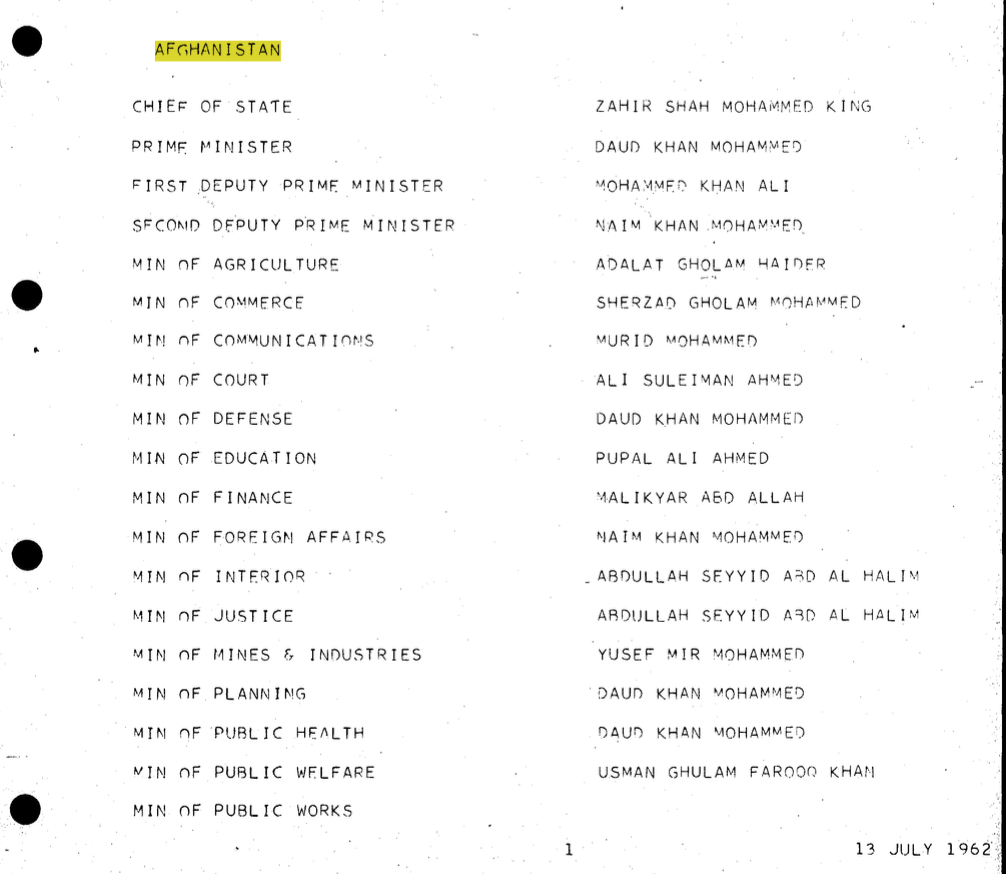
\includegraphics[scale=0.17]{figures/ocr-example-cia1.png} &

\includegraphics[scale=0.15]{figures/ocr-example-cia2.png}
\end{array}$
\end{center}
\caption{CIA Reports Tracking Political Transitions}
\end{figure}

\end{frame}
%%%%%%%%%%%%%%%%%%%%%%%%%%%%%%%%%%%%%%%%%%%%%%%%%%%%%%%%%%%%%%%%%%%%%%%%%


%%%%%%%%%%%%%%%%%%%%%%%%%%
\begin{frame}[fragile]{Measuring Political Turnover: Raw CIA data}
\begin{figure}[h]
\begin{center}$
\begin{array}{cc}
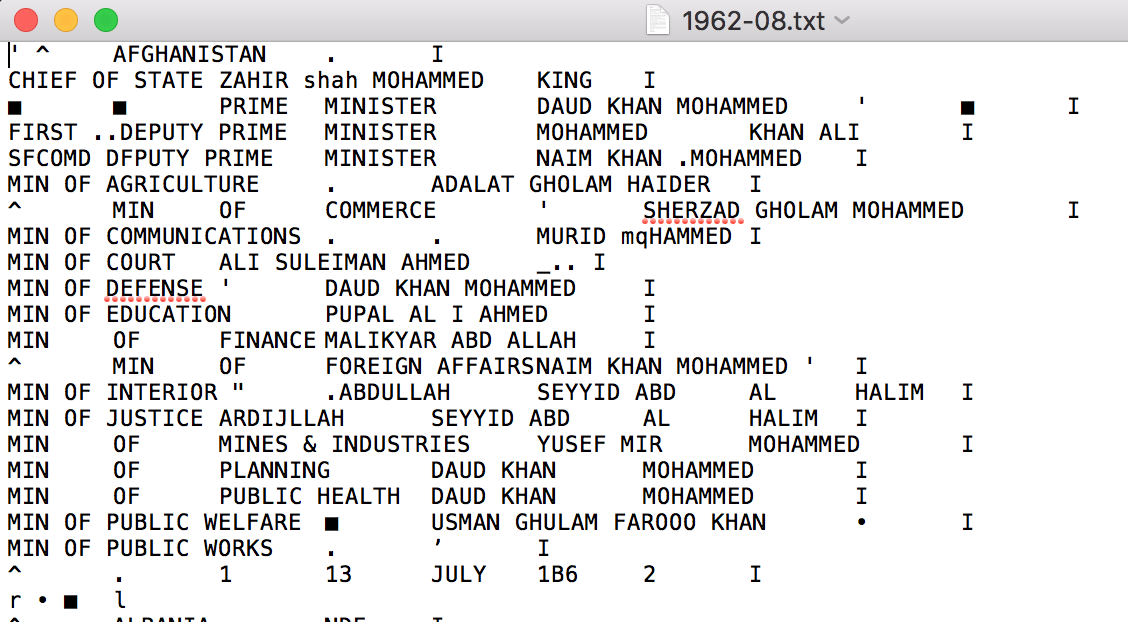
\includegraphics[scale=0.3]{figures/ocr-scan1.png} &
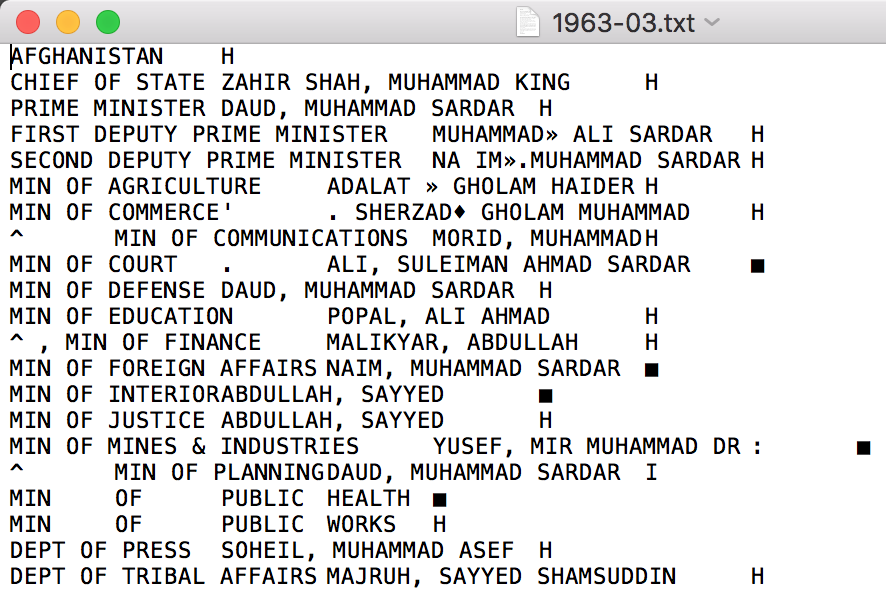
\includegraphics[scale=0.3]{figures/ocr-scan2.png}
\end{array}$
\end{center}
\caption{CIA Reports Tracking Political Transitions}
\end{figure}

$\Rightarrow$ 50 years of monthly data, essentially covering all countries of the world.
$\Rightarrow$ 3 million rows of raw data, initially 342,540 unique rows.
$\Rightarrow$ Levenshtein based dimensionality reduction reduces this down to 199,028.

\end{frame}
%%%%%%%%%%%%%%%%%%%%%%%%%%%%%%%%%%%%%%%%%%%%%%%%%%%%%%%%%%%%%%%%%%%%%%%%%


%%%%%%%%%%%%%%%%%%%%%%%%%%
\begin{frame}[fragile]{Measuring Political Turnover: Raw CIA data}
 It is evident that many strings are very very similar, and since typos are idiosyncratic to an individual document, we can take a frequentist approach.

\begin{knitrout}\tiny
\definecolor{shadecolor}{rgb}{0.969, 0.969, 0.969}\color{fgcolor}\begin{kframe}
\begin{alltt}
\hlkwd{library}\hlstd{(RecordLinkage)}
\hlkwd{levenshteinDist}\hlstd{(} \hlstr{"MIN OF EDUCATION	PUPAL AL I AHMED	I"}\hlstd{,}\hlstr{"MIN OF EDUCATION	POPAL, ALI AHMAD H"}\hlstd{)}
\end{alltt}
\begin{verbatim}
## [1] 6
\end{verbatim}
\begin{alltt}
\hlkwd{levenshteinSim}\hlstd{(}\hlstr{"MIN OF EDUCATION	PUPAL AL I AHMED	I"}\hlstd{,}\hlstr{"MIN OF EDUCATION	POPAL, ALI AHMAD H"}\hlstd{)}
\end{alltt}
\begin{verbatim}
## [1] 0.829
\end{verbatim}
\begin{alltt}
\hlcom{##run on whole vector}
\hlstd{VEC}\hlkwb{<-}\hlkwd{c}\hlstd{(}\hlstr{"CHIEF OF STATE	ZAHIR SHAH, MUHAMMAD KING	H"}\hlstd{,}\hlstr{"PRIME MINISTER	DAUD, MUHAMMAD SARDAR	H"}\hlstd{,}\hlstr{"FIRST DEPUTY PRIME MINISTER	MUHAMMAD» ALI SARDAR	H"}\hlstd{,}\hlstr{"SECOND DEPUTY PRIME MINISTER	NA IM».MUHAMMAD SARDAR	H"}\hlstd{,}\hlstr{"MIN OF AGRICULTURE	ADALAT » GHOLAM HAIDER	H"}\hlstd{,}\hlstr{"MIN OF COMMERCE	'	. SHERZAD♦ GHOLAM MUHAMMAD	H"}\hlstd{,}\hlstr{"^	MIN OF COMMUNICATIONS	MORID, MUHAMMAD	H"}\hlstd{,}\hlstr{"MIN OF COURT	.	ALI, SULEIMAN AHMAD SARDAR	■"}\hlstd{,}\hlstr{"MIN OF DEFENSE	DAUD, MUHAMMAD SARDAR	H"}\hlstd{,}\hlstr{"MIN OF EDUCATION	POPAL, ALI AHMAD	H"}\hlstd{,}\hlstr{"^ , MIN OF FINANCE	MALIKYAR, ABDULLAH	H"}\hlstd{,}\hlstr{"MIN OF FOREIGN AFFAIRS	NAIM, MUHAMMAD SARDAR	■"}\hlstd{,}\hlstr{"MIN OF INTERIOR	ABDULLAH, SAYYED	■"}\hlstd{,}\hlstr{"MIN OF JUSTICE	ABDULLAH, SAYYED	H"}\hlstd{,}\hlstr{"MIN OF MINES & INDUSTRIES	YUSEF, MIR MUHAMMAD DR	:	■"}\hlstd{,}\hlstr{"^	MIN OF PLANNING	DAUD, MUHAMMAD SARDAR	I"}\hlstd{,}\hlstr{"MIN	OF	PUBLIC	HEALTH	■"}\hlstd{,}\hlstr{"MIN	OF	PUBLIC	WORKS	H"}\hlstd{,}\hlstr{"DEPT OF PRESS	SOHEIL, MUHAMMAD ASEF	H"}\hlstd{,}\hlstr{"DEPT OF TRIBAL AFFAIRS	MAJRUH, SAYYED SHAMSUDDIN	H"}\hlstd{)}
\hlstd{SIM}\hlkwb{<-}\hlkwd{levenshteinSim}\hlstd{(}\hlstr{"MIN OF EDUCATION	PUPAL AL I AHMED	I"}\hlstd{,VEC)}

\hlstd{SIM}
\end{alltt}
\begin{verbatim}
##  [1] 0.262 0.211 0.260 0.189 0.372 0.304 0.439 0.326 0.342 0.857 0.256 0.304 0.400 0.486
## [15] 0.327 0.341 0.314 0.286 0.270 0.280
\end{verbatim}
\begin{alltt}
\hlstd{VEC[}\hlkwd{which.max}\hlstd{(SIM)]}
\end{alltt}
\begin{verbatim}
## [1] "MIN OF EDUCATION\tPOPAL, ALI AHMAD\tH"
\end{verbatim}
\end{kframe}
\end{knitrout}

\end{frame}
%%%%%%%%%%%%%%%%%%%%%%%%%%%%%%%%%%%%%%%%%%%%%%%%%%%%%%%%%%%%%%%%%%%%%%%%%


%%%%%%%%%%%%%%%%%%%%%%%%%%
\begin{frame}[fragile]{Clustering Based on Edit Distance}
Clustering is a very useful machine learning application that typically requires distance objects. Working with text data often requires a disambiguation of alternative spelling varations and clustering can be a very useful tool.

\begin{center}
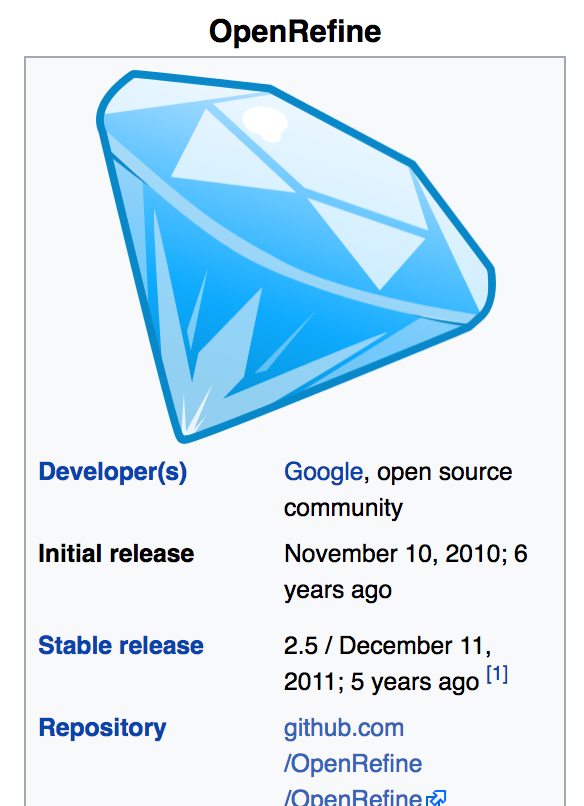
\includegraphics[scale=0.4]{figures/openrefine.png}
\end{center}


\end{frame}
%%%%%%%%%%%%%%%%%%%%%%%%%%%%%%%%%%%%%%%%%%%%%%%%%%%%%%%%%%%%%%%%%%%%%%%%%



%%%%%%%%%%%%%%%%%%%%%%%%%%
\begin{frame}[fragile]{OpenRefine Clustering}


\begin{center}
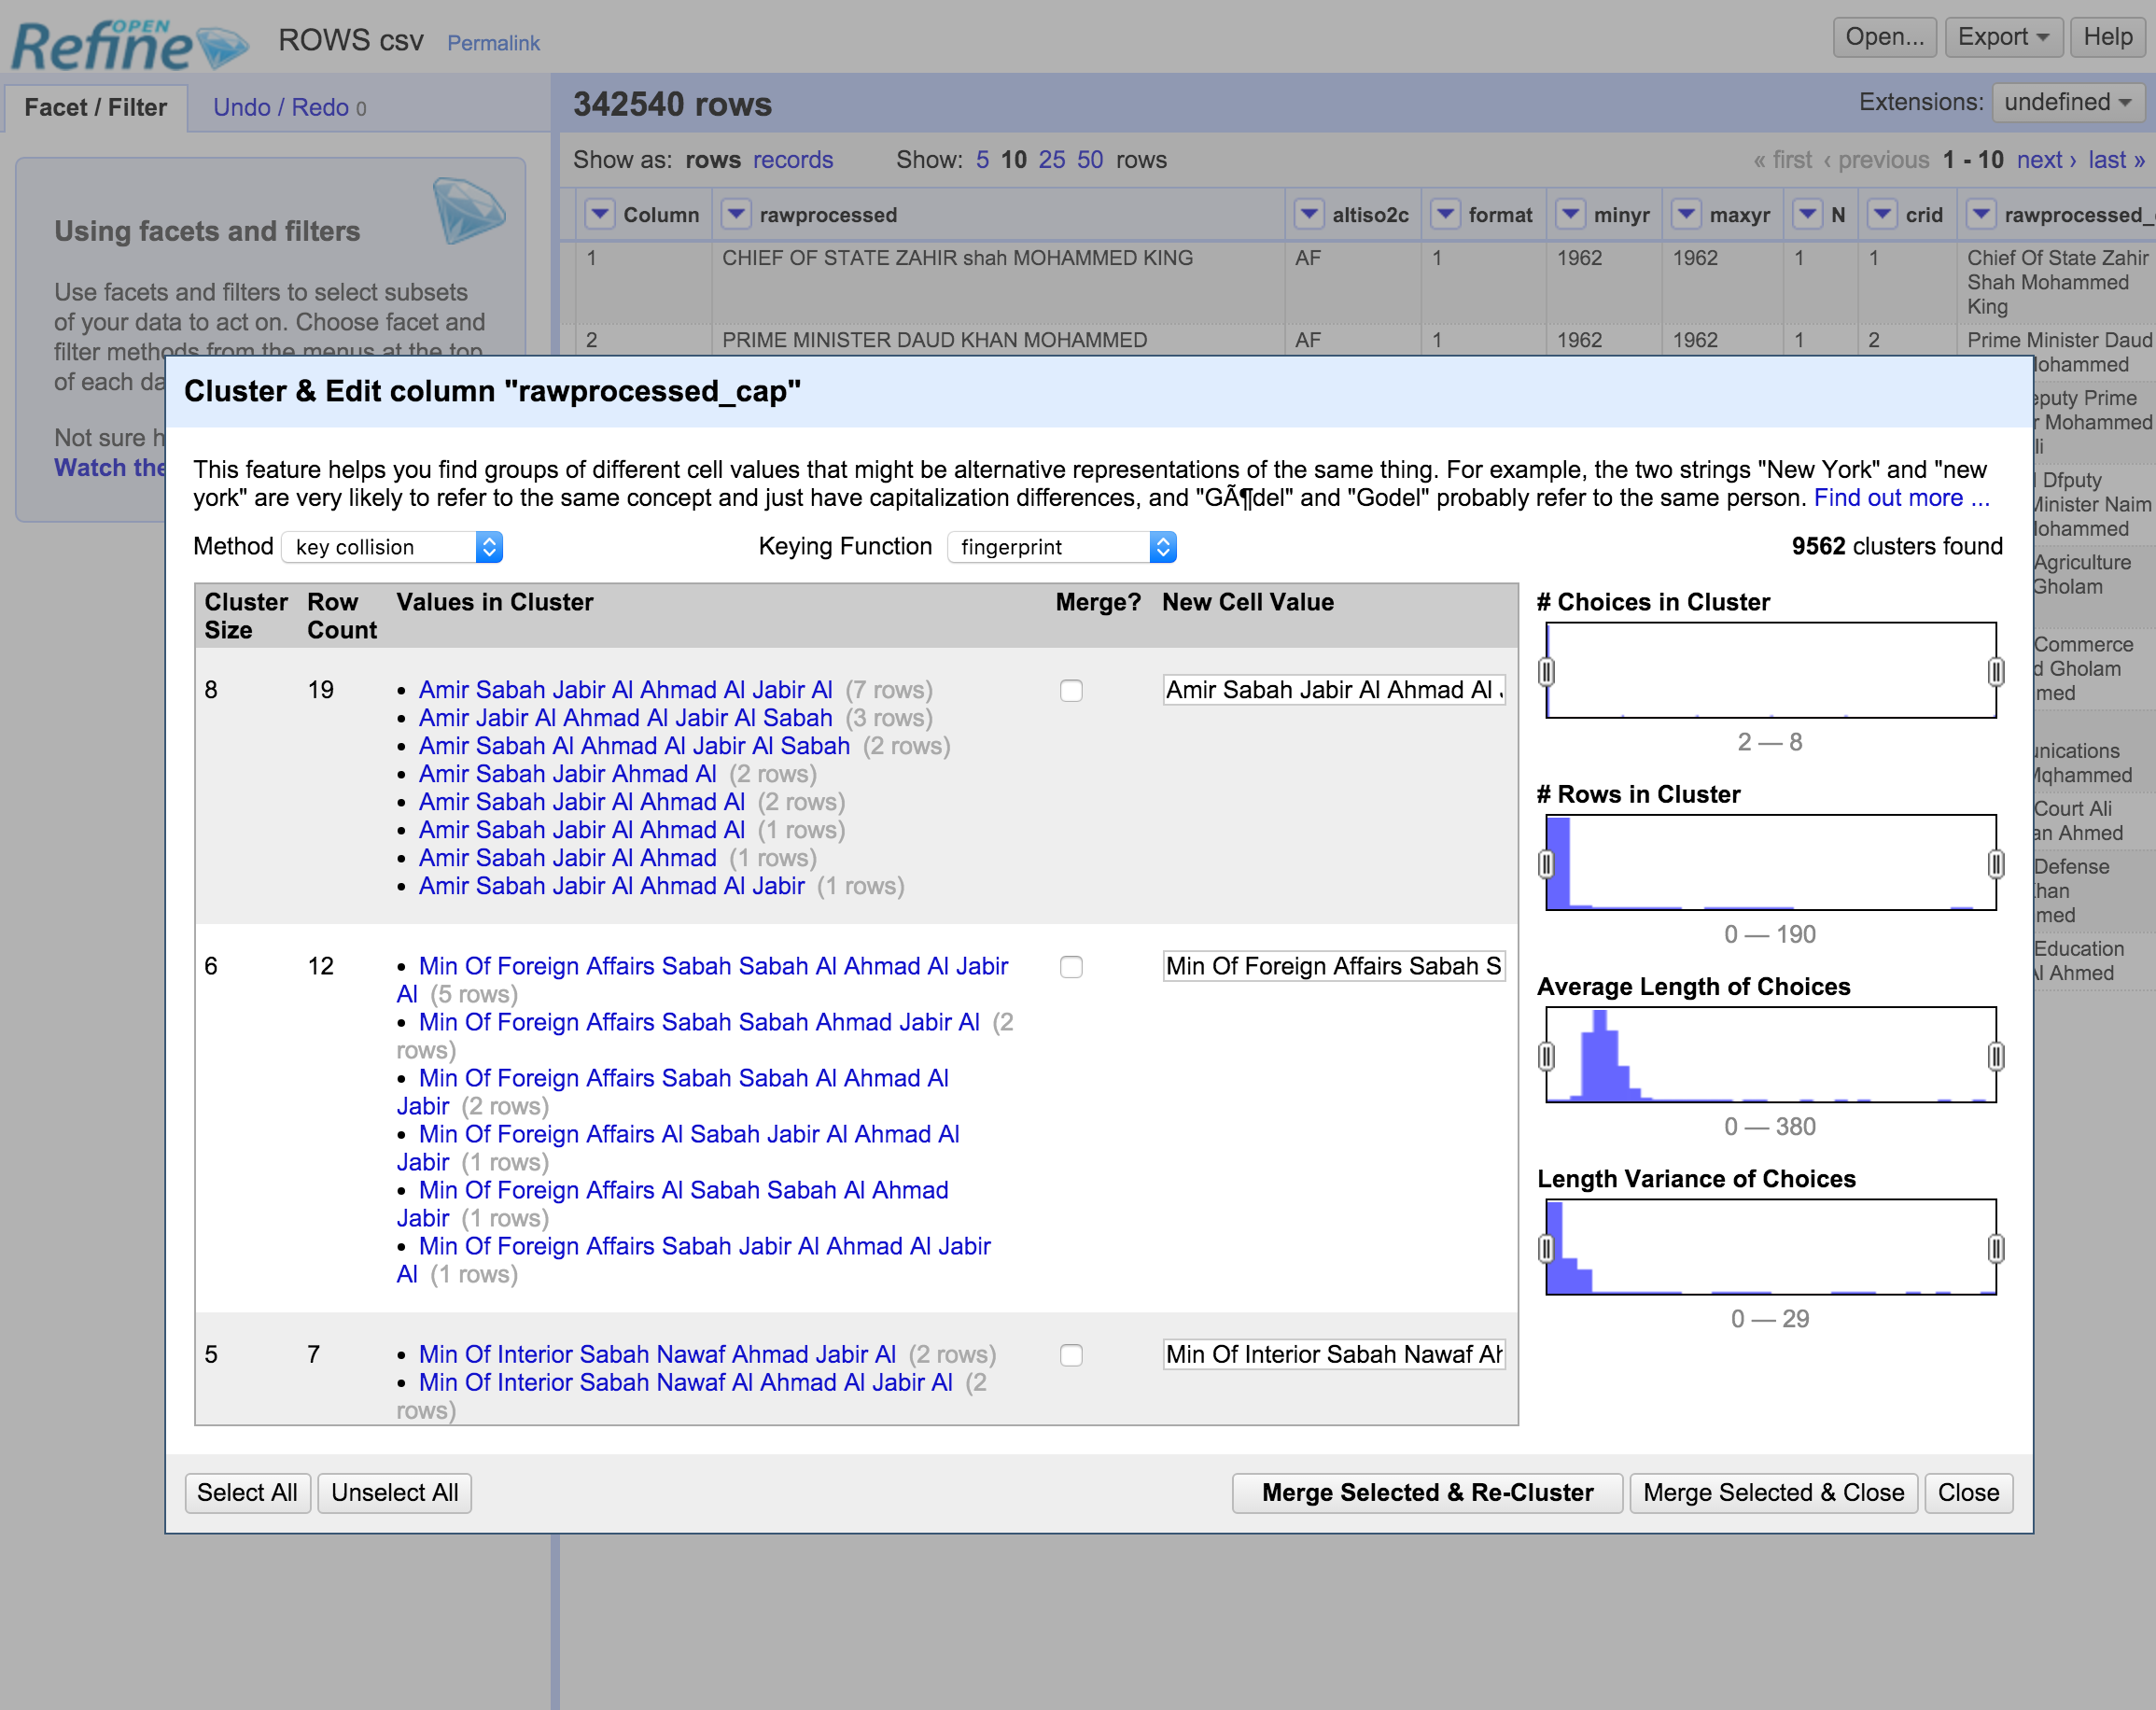
\includegraphics[scale=0.3]{figures/clustering-data-cleaning.png}
\end{center}


\end{frame}
%%%%%%%%%%%%%%%%%%%%%%%%%%%%%%%%%%%%%%%%%%%%%%%%%%%%%%%%%%%%%%%%%%%%%%%%%


\end{document}

